\documentclass[english, aip, jcp, priprint, graphicx,floatfix]{revtex4-1}
\usepackage{amsmath}
\usepackage{amsthm}
\usepackage{amssymb}
\usepackage{mathrsfs}
\usepackage{bbm,latexsym}
\usepackage{graphicx}
\usepackage{cancel}

%%%%%%%%%% Start TeXmacs macros
\catcode`\<=\active \def<{
\fontencoding{T1}\selectfont\symbol{60}\fontencoding{\encodingdefault}}
\catcode`\>=\active \def>{
\fontencoding{T1}\selectfont\symbol{62}\fontencoding{\encodingdefault}}
\newcommand{\mathd}{\mathrm{d}}
\newcommand{\nin}{\not\in}
\newcommand{\tmop}[1]{\ensuremath{\operatorname{#1}}}
\newcommand{\tmtextbf}[1]{{\bfseries{#1}}}
\newtheorem{definition}{Definition}
\newtheorem{proposition}{Proposition}
\newtheorem{theorem}{Theorem}
\newtheorem{lemma}{Lemma}
\newtheorem{algorithm}{Algorithm}
%%%%%%%%%% End TeXmacs macros

\draft % marks overfull lines with a black rule on the right

\theoremstyle{plain}
\newtheorem{thm}{\protect\theoremname}
\newtheorem*{thm*}{\protect\theoremname}
\theoremstyle{definition}
\newtheorem{defn}[thm]{\protect\definitionname}
\theoremstyle{plain}
\newtheorem{cor}[thm]{\protect\corollaryname}

\global\long\def\dimension{{\mathfrak{n}}}


\usepackage{babel}
\providecommand{\corollaryname}{Corollary}
\providecommand{\definitionname}{Definition}
\providecommand{\lemmaname}{Lemma}
\providecommand{\theoremname}{Theorem}

\begin{document}

\title{Overcoming Entropic Barriers by Capacity Hopping} %Title of paper

\author{Jackson Loper}
\thanks{These two authors contributed equally}
\affiliation{Data Science Institute, Columbia University, New York, NY, USA}

\author{Guangyao Zhou}
\thanks{These two authors contributed equally}

\author{Stuart Geman}

\affiliation{Division of Applied Mathematics, Brown University, Providence, RI, USA}
\date{\today}

\begin{abstract}
	We present Capacity Hopping (CHop), a method for estimating hitting probabilities of small targets in molecular dynamics simulations. Reaching small targets out of a vast number of possible configurations consitute an \emph{entropic barrier}. Experimental evidence suggests that entropic barriers are ubiquitous in biomolecular systems, and often characterize the rate-limiting step of biomolecular processes. CHop provides valuable information in the presence of entropic barriers. It is based on a novel theoretical analysis of hitting probabilities in the presence of entropic barriers; we show that in many cases the hitting probabilities are approximately invariant to the initial condition, as long as the intitial condition is modestly far away from the targets.  Given this invariance, we show that the hitting probabilities must also be invariant to the energy landscape away from the target sets, and can be well-approximated in terms of ``capacities" of local sets around the targets.  Using these theoretical results and a new capacity estimation algorithm, we develop CHop, a method for estimating the approximately constant hitting probabilities. Numerical experiments on a toy model with a golf-course potential show that CHop is nearly as accurate as naive simulations in estimating hitting probabilities, but 750 times faster.
\end{abstract}

\pacs{}% insert suggested PACS numbers in braces on next line

\maketitle %\maketitle must follow title, authors, abstract and \pacs

\global\long\def\TODOTHIS{{\huge !!!!}}

\global\long\def\indicatorf#1{\mathbb{I}_{#1}}
\global\long\def\capac#1#2{\mathrm{cap}\left(#1;#2\right)}
\global\long\def\fnsp{\mathscr{H}^1}
\global\long\def\bb#1{\mathcal{B}\left(#1\right)}
\global\long\def\BB#1{\mathcal{\bar B}\left(#1\right)}

\section{Introduction}

Molecular dynamics simulations help us understand a diverse range of biomolecular processes, including the folding of macromolecules into their native configurations\cite{Scheraga2007-qw} and the conformational changes involved in their functioning.\cite{Hospital2015-ol} Since their first introduction in the 1970s,\cite{McCammon1977-kg, Warshel1976-qg} substantial increase in speed and accuracy of molecular dynamics simulations has been achieved. However, we are still severely limited in the timescale we can access. Even with specialized hardwares, we can only achieve atomic-level simulations on timescales as long as milliseconds,\cite{Dror2012-ws} while the timescales for various biomolecular processes vary widely, and can last for seconds or longer.\cite{Naganathan2005-ki, Zemora2010-lb} 

Efforts have been made to extend the timescale accessible by molecular dynamics simulations from two distinct perspectives: A \emph{kinetic perspective} seeks to find ways to directly understand the dynamics and simulate them with less computational effort, usually under the framework of kinetic transition networks\cite{Noe2006-cs, Wales2006-ur} or Markov State Models\cite{Pande2010-yi, Chodera2014-bh, Husic2018-xp}. The reaction rates are given by various methods that build on top of transition state theory\cite{Eyring1935-ur, Chandler1978-bq, Wigner1997-kk}, including transition path sampling\cite{Dellago1998-lb, Bolhuis2002-ws}, transition interface sampling\cite{Van_Erp2005-vw}, and transition path theory\cite{E2006-fm, E2010-sr}. By constrast, a \emph{thermodynamic perspective} aims to understand and efficiently sample from the ``equilibrium distribution'' on the configuration space; simulated annealing,\cite{Kirkpatrick1983-su} genetic algorithms\cite{Goldberg1989-ko} and parallel tempering\cite{Sugita1999-vh} are representative examples of this approach. However, dynamics is destroyed in these methods, and additional work\cite{Yang2007-gn, Andrec2005-fh, Zheng2009-ow, Huang2010-uu} is needed in order to recover the kinetic information of the system.

In this paper we will focus on the \emph{hitting probability question}: ``Given an initial condition $X_0$ and two target sets, $A,B$, what is the probability that we will hit target $A$ first?'' This question lies in-between the two different perspectives. Compared with the thermodynamic perspective, it adds certain dynamic information in that we can obtain sequences of \emph{key configurations} from the hitting probabilities. Compared with the kinetic perspective, it lacks certain dynamic information in that we are interested not in \emph{how long} it takes to hit each target, but only in the probability that we hit one target first. The \emph{hitting probability question} by itself can help us understand certain kinetic aspects of the system, e.g. important intermediates and folding pathways in the context of folding, by looking at sequences of key configurations visited in the simulations; it also appears as an important subproblem for other methods, e.g. transition probability estimation in Markov State Models, commitor function estimation in transition path theory, etc..

We are especially interested in the ``small-target" regime for the \emph{hitting probability question}, where we try to reach small targets out of a vast number of possible configurations. This constitutes an \emph{entropic barrier}. A prototypical example is regions on the energy landscape with ``golf-course'' potentials.\cite{bicout2000entropic, Baum1986-we, Wille1987-tf}. These potentials commonly take place in high-dimensional configuration spaces. They feature a large region and several small targets within the region.  Away from the targets, the potential energy is relatively flat.  Near the targets, the potential energy may be complicated. Regions on the energy landscape with these small-target golf-course potentials are ubiquitous in biomolecular systems. Folding-like dynamics (such as RNA folding or protein folding) are one prominent example, where it is thought that ``folding rates are controlled by the rate of diffusion of pieces of the open coil in their search for favorable contacts'' and ``the vast majority of the space covered by the energy landscape must actually be flat.''\cite{McLeish2005-dq} Experimental evidence shows that exploration of regions with golf-course potentials forms the rate-limiting step for a variety of processes.\cite{Teschner1987-qs, Jacob1999-bs, Goldberg1999-mv, Plaxco1998-iv}

Direct simulations offer one way to estimate hitting probabilities, but perform poorly in the presence of entropic barriers. If the targets are very small, it may take a long time for the process to find either target.  It will thus require significant  computational effort to directly simulate an entire trajectory. In general, the computational efficiency of direct simulations will scale inversely with the size of the targets.

Standard acceleration techniques do not always apply in the presence of entropic barriers.  For example, simulated annealing and parallel tempering work poorly in the presence of regions with golf-course potentials.\cite{Baum1986-we, Wille1987-tf, Machta2009-gh} Some authors take a pessimistic view on this subject: ``If these processes are intrinsically slow, i.e. require an extensive sampling of state space'' (which is indeed the case in the presence of entropic barriers), ``not much can be done to speed up their simulation without destroying the dynamics of the system.''\cite{Christen2008-ge}

In this paper, we argue for a new point of view: the long timescales in the presence of entropic barriers can be a blessing rather than a curse.  If the targets are sufficiently small, the system may reach temporary equilibrium before it hits one of the targets. The exact initial condition within the region may become irrelevant. As a consequence, the hitting probabilities might be approximately constant for nearly all initial conditions in the region.  Moreover, the hitting probabilities may be approximately \emph{invariant} to the energy landscape away from the targets, meaning we can compute the approximately constant hitting probabilities using only local simulations around the targets.

The contributions of this paper are as follows: 

\begin{description}
	\item[Theory of golf-course potentials] We analyze regions with golf-course potentials (a special case of entropic barriers) to show that the hitting probabilities are approximately invariant to the initial condition, as long as the initial condition is modestly far away from the target. We point the way to proving similar results for other entropic barriers.
	\item[Theory of invariant hitting probabilities] Given approximate invariance to initial conditions, we show that the hitting probabilities are also approximately invariant to the energy landscape away from the target regions. In particular, we demonstrate that the hitting probabilities can be accurately estimated using only local information around the targets, coming in the form of ``capacities".
	\item[Application] Inspired by the theoretical results, we present CHop as a general method to estimate hitting probabilities in the presence of entropic barriers. We verify the effectiveness of CHop through extensive numerical experiments.
\end{description}

The rest of the paper is organized as follows. In Section \ref{sec:toy_model}, we present a toy model with a golf-course potential.  This example will run across the entire paper as a central thread for our theoretical and numerical analysis. In Section \ref{sec:model_formulation}, we present our theoretical results. We define $\varepsilon$-flatness to capture the idea that hitting probabilities are approximately invariant to the initial condition, as long as the initial condition is away from the targets.  In Theorem \ref{thm:epsilon_flat} we then establish the $\varepsilon$-flatness of the toy model. Finally, in Corollary \ref{thm:main_cor} we show the consequences of the $\varepsilon$-flatness condition for for general stationary reversible SDEs: hitting probabilities for initial conditions away from the targets can be approximated using local capacities, with an error of roughly $\sqrt\varepsilon$.  Thus these hitting probabilities are approximately invariant to the energy landscape away from the targets.  In Section \ref{sec:algorithm}, we talk about applications. We propose CHop as a general method for estimating hitting probabilities in the presence of entropic barriers, and discuss the central computational issue of CHop: the efficient estimation of the capacities. We present extensive numerical experiments and results in Section \ref{sec:experiments} to demonstrate the effectiveness of CHop, before giving conclusions and future directions in Section \ref{sec:conclusion}.


\section{A Toy Model}\label{sec:toy_model}

To concretely demonstrate the CHop method, we introduce a simple toy model with a golf-course potential.  This model features a high-dimensional configuration space containing two small target regions, $A$ and $B$.  Away from the targets, the potential energy is completely flat.  To further simplify the analysis and facilitate numerical validation, we will assume all sets of interest are spheres.  The resulting model is perhaps the simplest possible example of a dynamics with golf-course qualities.  

We will now give a formal definition of the model.  The dynamics will take place inside the unit ball, $\Omega = \bb{0,1}\subset \mathbb{R}^\dimension$, where $\bb{x, r} \triangleq \{ y : || y - x || < r \}$.  The configuration space will also feature two important target regions:
\begin{align*}
A &\triangleq \bb {x_A, r_A}\\
B &\triangleq \bb {x_B, r_B}
\end{align*}
where $x_A,x_B \in \Omega$.  Given an initial condition $X_0\in \Omega \backslash (A\cup B)$, we will be be interested to know whether the dynamics carry the system into $A$ or $B$ first.  These dynamics will be defined in terms of a $d$-dimensional Brownian motion $W_t$, according to 
\begin{equation} \label{equ:toy_sde}
\mathrm{d} X_t = - \nabla U (X_t) \mathrm{d} t + \mathrm{d} W_t 
\end{equation}
with reflecting boundary at the boundary of $\Omega$.  We will require that the potential energy $U$ is differentiable and flat outside of a region around the targets.  In particular, we will fix $d_A>r_A$ and $d_B>d_B$ and require that $U (x) = 0, \forall x \not\in \bb{x_A,d_A} \cup \bb{x_B,x_B}$.  To simplify the theorems, we also require that the surface of $\Omega$ is part of the flat region, i.e. $||x_A||+d_A,||x_B|+d_B<1$.  We also assume that the two target regions do not overlap: $\BB{x_A,d_A},\BB{x_B,x_B}$ are disjoint, where $\BB{}$ denotes the closure of $\bb{}$.  

This toy model encapsulates the essential characteristics of entropic effects: if $r_A, r_B$ are small, the trajectory of $X$ will generally be spent well away from $A$ or $B$, in the large flat region of the energy landscape that separates $A$ from $B$. The nontrivial energy landscapes in the immediate vicinity of $A$ and $B$ reflect the local nature of energetic interactions in the system under biological conditions, and the reflecting boundary $\partial\Omega$ captures the notion that not all configurations for the biomolecular system are sensible, because of, for example, the limits on bond lengths, angles and dihedral angles in the case of RNA molecules.

\section{Theory: $\varepsilon$-flatness and CHop Probabilities}\label{sec:model_formulation}

With this toy model in mind, we now turn to the general results of this paper. In general, we will assume the underlying physical process governing the macromolecule is a stationary reversible diffusion process in the configuration space $\Omega$, with invariant
measure ${\mu}= e^{- U (x)} \mathrm{d} x$.  In particular, the dynamics will be defined in terms of a $d$-dimensional Brownian motion $W_t$, according to 
\begin{equation}\label{equ:general_sde}\mathrm{d} X_t = b (X_t) \mathrm{d} t + \sigma (X_t) \mathrm{d} W_t \end{equation}
where $b: \Omega \rightarrow \mathbbm{R}^\dimension$ and $\sigma :
\Omega \rightarrow \mathbbm{R}^{\dimension \times m}$ are differentiable vector-valued
and matrix-valued functions.  We refer the reader to Appendix \ref{sec:reversible_diffusion} for a detailed account of stationary reversible diffusion processes.

As in the toy model, we will be interested in two target regions, $A,B\subset \Omega$.  Given an initial condition $X_0\in \Omega \backslash (A\cup B)$, we will be be interested to know whether the dynamics carry the system into $A$ or $B$ first.  That is, we are interested in the hitting probabilities
\[ h_{A, B}(x) \triangleq \mathbb{P}(X_{\tau_{A\cup B}}\in A|X_0=x)\]
where $\tau_S$ indicates the time when the process first hits a set $S$, i.e. $\tau_S \triangleq \inf \{ t \geqslant 0 : X_t \in S \}$.  Thus $h_{A,B}(x)$ indicates the probability that $\{X_t\}_{t \geq 0}$ hits $A$ before $B$ given that it starts at $x\in\Omega$. 

Our theoretical inquiry began with an intuition.  Let us consider the case that $A$ and $B$ are very small relative to $\Omega$.  Let us also assume that $U$ is sufficiently flat in $\Omega / (A\cup B)$.  In this case, for any starting point $x\in \Omega / (A\cup B)$, we would reach local equilibrium before we hit the targets.  In that case the hitting probability $h_{A, B}(x)$ should not depend upon the initial condition.  That is, $h_{A,B}(x)$ should be approximately \emph{constant} for all initial conditions $x$ which are reasonably far away from $A$ and $B$.  In addition, since we reach local equilibrium before we hit the targets, the exact internal structure of $\Omega / (A\cup B)$ away from $A$ and $B$ may not be important.  We might therefore hope that the hitting probabilities could be accurately estimated without looking at this internal structure.  In summary, it seems that
%
\begin{enumerate}
    \item There should be some constant $\bar h$ such that $\bar h_{A,B} \approx h_{A,B}(x)$ for all initial conditions $x$ which are reasonably far away from $A$ and $B$.
    \item It should be possible to estimate $\bar h$ using only knowledge of the dynamics in the local regions around $A,B$.  
\end{enumerate}
%
In what follows, we make the above intuitions rigorous.  First, for our toy model we establish that the hitting probabilities are indeed constant away from $A,B$.  We see the kinds of arguments that would be necessary to establish this result for other models.  Second, we turn to the general case.   Whenever hitting probabilities are approximately constant in a region away from $A,B$, we show that the value of this constant can be determined by looking only at the dynamics of local regions around $A,B$.  In particular, we show that the key quantity is what is known as the ``capacity'' of local sets around the targets. 

\subsection{Approximately Constant Hitting Probability}

In this section, we introduce the concept of $\varepsilon$-flatness, establish it for our toy model, and see when it will hold in general models.  We introduce this concept to formally define what it would mean that the hitting probability function $h_{A, B}(x)$ is ``approximately constant'' in a given region.
%
\begin{definition}($\varepsilon$-flatness)\label{def:epsilon_flat}
For any function $h$ on $\Omega$ and an $\varepsilon > 0$, a set $M\subset \Omega$ is $\varepsilon$-flat for the function $h$ iff $\sup_{x, y \in M} | h (x) - h (y) | < \varepsilon$.
\end{definition}
%
Note that if $M$ is $\varepsilon$-flat for $h$, then we can always find some constant $\bar h$ so that $\sup_{x \in M}|\bar h-h(x)|<\varepsilon$ for all $x\in M$.  Simply pick $\bar h$ to be $h(x)$ for any $x\in M$.  

For the toy model, we can see how  $\varepsilon$-flatness applies to hitting probabilities.  Let us recall the notation of the toy model.  We have two sets, $A=\bb{x_A,r_A},B=\bb{x_B,r_B}$ in $d$-dimensional space.  The dynamics are governed by a potential energy which is flat outside of $\bb{x_A,d_A}\cup\bb{x_B,d_B}$, where $d_A>r_A,d_B>r_B$.  We now introduce a third layer of neighborhoods around the target regions.  We fix some $r_{\tilde A}>d_A,r_{\tilde B}>d_B$ and define $\tilde A=\bb{x_A,r_{\tilde A}},\tilde B=\bb{x_B,r_{\tilde B}}$.  We will show conditions such that the hitting probabilities are constant away from $\tilde A,\tilde B$.  In particular, the probabilities must be constant as long as when the targets $A, B$ are sufficiently small or the dimension is high:

\begin{theorem}\label{thm:epsilon_flat}
For any fixed value of the ambient dimension $\dimension \geq 3$ and any $r_{\tilde{A}}, r_{\tilde{B}}, \varepsilon > 0$, there exists a constant $c=c(\dimension, r_{\tilde{A}}, r_{\tilde{B}}, \varepsilon)$ such that if $d_{A}, d_{B} < c$ then $\bb {0, 1} / (\tilde{A} \cup \tilde{B})$ is $\varepsilon$-flat for the function $h_{A,B}(x)$.  Likewise for any fixed value of $d_{A}, r_{\tilde{A}}, d_{B}, r_{\tilde{B}}, \varepsilon>0$, there exists a constant $c=c(d_{A}, r_{\tilde{A}}, d_{B}, r_{\tilde{B}}, \varepsilon)$ such that if $\dimension \geq c$ then $\bb {0, 1} / (\tilde{A} \cup \tilde{B})$ is $\varepsilon$-flat for the function $h_{A,B}(x)$.
\end{theorem}

We defer the proof of this theorem to Appendix \ref{sec:proof_epsilon_flat}. Inspection of the proof demonstrates that the key for establishing $\varepsilon$-flatness is a proper separation of time scales: it takes a short time for the process $\{X_t\}_{t\geq 0}$ to reach local equilibrium in $\bb {0, 1} / (\tilde{A} \cup \tilde{B})$ and a long time for the process $\{X_t\}_{t\geq 0}$ to hit the targets $A$ and $B$.  Any model with these characteristics will feature $\varepsilon$-flat hitting probabilities.

\subsection{Estimating Constant Hitting Probability Using Local Information}

In this section, we show that hitting probabilities can be determined using only local information around the targets, as long as the hitting probability function enjoys $\varepsilon$-flatness.  In particular, it will be sufficient to calculate the ``capacities'' for local sets around the targets.  This is defined as follows.  Let $\{X_t\}_{t\geq 0}$ be a reversible stationary process governed by Equation (\ref{equ:general_sde}).  Then for $A \subset \tilde{A} \subset \Omega$, the capacity $\ensuremath{\operatorname{cap}} (A, \tilde{A})$ for $X$ is defined as
%
\[ \ensuremath{\operatorname{cap}} (A, \tilde{A}) \triangleq \frac{1}{2} \int_{\Omega}
||\sigma(x) \nabla h_{A, \tilde{A}^c}(x)||^2 e^{- U(x)} \mathrm{d} x \]
%
Recall that $h_{A, \tilde{A}^c}(x)$ denotes the probability that the dynamics will hit $A$ before hitting $\tilde{A}^c$, given that $X_0=x \in \tilde A\backslash A$.  We refer the reader to Appendix \ref{sec:reversible_diffusion} for more details on capacity and the the related concept of Dirichlet form.

In the presence of $\varepsilon$-flatness, these capacities are intimately related to hitting probabilities:

\begin{theorem}\label{thm:main_thm}  Let $\{X_t\}_{t\geq 0}$ be a reversible stationary diffusion on $\Omega$ governed by Equation (\ref{equ:general_sde}).  Let $A\subset\tilde A\subset\Omega,B\subset\tilde B\subset\Omega$.  If $\tilde A,\tilde B$ are disjoint and $\Omega \backslash (\tilde A \cup \tilde B)$ is $\varepsilon$-flat for the hitting probabilities $h_{A,B}(x)$, then 
\[ \sup_{x \in M} \left| h_{A,B} (x) - \frac{\ensuremath{\operatorname{cap}} (A,
\tilde{A})}{\ensuremath{\operatorname{cap}} (A, \tilde{A})
+\ensuremath{\operatorname{cap}} (B, \tilde{B})} \right| \leqslant
\varepsilon + \sqrt{\frac{\varepsilon}{2}} \]
for any $\varepsilon \in[0,2/9]$.
\end{theorem}

We defer the proof to Appendix \ref{sec:proof_thm}. This theorem generalizes naturally to the case of multiple targets.  For a collection of targets with neighborhoods, we first define the approximate probability estimates, which we call ``CHop probabilities.''

\begin{definition}
Let $\{X_t\}_{t\geq 0}$ be a stationary reversible diffusion process on $\Omega$.  Pick $A_1\cdots A_n \subset \Omega$ and $\tilde A_1\cdots \tilde A_n \subset \Omega$ such that $A_k \subset \tilde A_k$.  Then the \textbf{CHop Probability} for the set $A_k$ (given all the other sets $A_1\cdots, A_{k-1}, A_{k+1}, \cdots A_n \subset \Omega$ and $\tilde A_1\cdots \tilde A_n \subset \Omega$) is given by
\begin{equation*}
p_{A_k} = \frac{\ensuremath{\operatorname{cap}} (A_k, \tilde{A}_k)}{\sum_{i = 1}^n \ensuremath{\operatorname{cap}} (A_i, \tilde{A}_i)}, k=1,\dots, n
\end{equation*} 
\end{definition}

In terms of these definitions, Theorem \ref{thm:main_thm} then yields:

\begin{cor}\label{thm:main_cor} Let $u_k = h_{A_k,\cup_{i\neq k} A_i}$ denote the probability the process hits $A_k$ before the other target sets.  Fix any $\varepsilon \in \left( 0, \frac{2}{9} \right]$.  If $M = \Omega \backslash \bigcup_{k = 1}^n \tilde{A}_k $ is $\varepsilon$-flat for the functions $\{u_k\}_{k\in1,\dots, n}$ then each $u_k$ is well-approximated by the corresponding CHop Probability:
\[ \sup_{x \in M} \left| u_k (x) - p_{A_k} \right| \leqslant \varepsilon + \sqrt{\frac{\varepsilon}{2}}, k=1,\dots, n\]
\end{cor}

This corollary follows immediately from Theorem \ref{thm:main_thm} and additivity of the capacity (Proposition \ref{prop:capacity} in Appendix \ref{sec:reversible_diffusion}). 

\section{Application: CHop Method and Capacity Estimation}\label{sec:algorithm}

Inspired by the theoretical analysis above, we introduce the CHop method as a way to study kinetic aspects of biomolecular systems by efficiently dealing with regions with golf-course potential. We present the high-level idea of the CHop method, and give a detailed account of the key computational issue of the CHop method, the efficient estimation of capacities. A general framework based on a simple lemma is given for capacity estimation, and the associated challenges are discussed. To demonstrate this framework, we give an outline of a flexible and general-purpose algorithm for capacity estimation, and make some concrete choices to show how exactly the algorithm works in the case of our toy model. This will serve as the basis for the numerical experiments and results in Section \ref{sec:experiments}.

Recall that in the previous section on theory, we made the following two key points:

\begin{enumerate}
    \item We can establish $\varepsilon$-flatness in regions with a golf-course potential, and the hitting probabilities of the various targets remains approximately a constant over a large part of the flat region.
    \item The approximately constant hitting probabilities can be accurately estimated using CHop probabilities, which depend on capacities that can be determined solely based on the local information around the targets.
\end{enumerate}

The above theoretical insights provide us with an efficient way to deal with golf-course potentials, so that we can get information of the biomolecular system on a much longer time-scale: we make use of our knowledge of the targets (which is typically available, e.g. in the form of different secondary structures for RNAs) to carry out local simulations around the targets for the estimation of capacites. Capacities can then be used to calculate the CHop probabilities, which give us an accurate estimate of the approximately constant hitting probabilities. This enables us to study kinetics of the biomolecular systems by looking at sequences of key configurations visited in molecular dynamics simulations, which is the essence of the CHop method.

\subsection{CHop Method}

Let $\{X_t\}_{t \geq 0}$ by a process governed by Equation \ref{equ:general_sde} on $\Omega$.  Let $A_1\cdots A_n \subset \Omega$ denote the target sets of interest.  On a high-level, the CHop method is a method for approximating hitting probabilities for systems initialized inside large, flat regions.  It consists of the following steps:

\begin{enumerate}
    \item Identify suitable sets $\tilde A_k \subset \Omega$ where $A_k \subset \tilde{A}_k, k=1, \cdots, n$, such that we can establish the $\varepsilon$-flatness of $M = \Omega \backslash \bigcup_{k = 1}^n \tilde{A}_k $ for hitting probability functions $h_{A_k,\cup_{i\neq k} A_i}(x)$.
    \item Estimate the capacities $\ensuremath{\operatorname{cap}} (A_k, \tilde{A}_k)$, from which we can derive the CHop probabilities
\begin{equation*}
p_{A_k} = \frac{\ensuremath{\operatorname{cap}} (A_k, \tilde{A}_k)}{\sum_{i = 1}^n \ensuremath{\operatorname{cap}} (A_i, \tilde{A}_i)}, k=1,\dots, n
\end{equation*} 
    \item For any initial condition $x \in M$, approximate the hitting probability $h_{A_k,\cup_{i\neq k} A_i}(x)$ with the CHop probability $p_{A_k}$.  
\end{enumerate}

To make the CHop method practical, we need to be able to estimate the capacities accurately and efficiently. This would be our topic for the rest of this section.

\subsection{Estimation of Capacities}

We start our discussion on estimating the capacities with a simple lemma:
\begin{lemma}\label{thm:capacity_lemma}
For a stationary reversible  diffusion process $X_t$ in $\Omega$ with
invariant measure ${\mu}= e^{- U (x)} \mathrm{d} x$ and diffusion matrix
$a (x)$, given non-empty sets $A \subset G \subset \tilde{G} \subset
\tilde{A}$ with smooth boundaries, the capacity
$\ensuremath{\operatorname{cap}} (A, \tilde{A})$ can be calculated by
\begin{eqnarray*}
\ensuremath{\operatorname{cap}} (A, \tilde{A}) & = & \int_{\partial
\tilde{G}}  h_{A,
\tilde{A}^c} (x) e^{- U (x)} [a (x) \nabla h_{G, \tilde{G}^c} (x)]^T \textbf{n} (x)\mathd S\\
&   & - \int_{\partial G}  h_{A, \tilde{A}^c} (x) e^{- U (x)} [a (x) \nabla h_{G, \tilde{G}^c} (x)]^T \textbf{n} (x)\mathd S
\end{eqnarray*}
where ${\textbf{n}} (x)$ in the integral is taken as the outward-facing normal vector at point $x$ on the surface we are integrating on, and $\mathd S$ represents the surface integral.
\end{lemma}

We defer the proof of this lemma to Appendix \ref{sec:proof_lemma}. This lemma provides us with a general framework for estimating the capacities.   In particular, we can approximate the integrals in the lemma with a Monte Carlo method, as long as we can overcome three challenges:
\begin{enumerate}
    \item To sample $y_1,y_2,\cdots y_m$ on $\partial G$ and $\tilde y_1,\tilde y_2 \cdots \tilde y_n$ on $\partial \tilde{G}$ according to the invariant measure $e^{- U(x)}\mathrm{d}x$ restricted on $\partial G, \partial \tilde{G}$ and compute the surface areas $|\partial G|$ and $|\partial \tilde G|$

\item To estimate $\nabla h_{G, \tilde{G}^c}$ on $\partial G$ and
$\partial \tilde{G}$

\item To estimate $h_{A, \tilde{A}^c}$ on $\partial G$ and $\partial
\tilde{G}$
\end{enumerate}
With these pieces in place, using the lemma, we can approximate the capacity by
\begin{gather}\label{eq:capesteq}
\begin{array}{cc}
\ensuremath{\operatorname{cap}} (A, \tilde{A}) \approx & 
|\partial \tilde G|\frac{\sum_i^n h_{A,\tilde A^c}(\tilde y_i)[a(\tilde y_i)\nabla h_{G,\tilde G^c}(\tilde y_i)]^T \textbf{n}(\tilde y_i)}{\sum_i^n e^{U(\tilde y_i)}} \\
& - |\partial G|\frac{\sum_i^m h_{A,\tilde A^c}(y_i)[a(y_i)\nabla h_{G,\tilde G^c}(y_i)]^T \textbf{n}(y_i)}{\sum_i^n e^{U(y_i)}} 
\end{array}
\end{gather}

The first challenge (sampling of points) can be addressed using existing methods, e.g. an importance sampling based approach, and is further simplified by the fact that we have the freedom to pick $G$ and $\tilde{G}$. In some special cases (e.g. the toy model), it's not hard to pick $G, \tilde{G}$ in such a way that we can get exact samples from the invariant measure $e^{- U (x)} \mathrm{d} x$.

The second challenge (estimation of $h_{G,\tilde G}$) can be addressed by making judicious choice of $G$ and
$\tilde{G}$ so that $\nabla h_{G, \tilde{G}^c}$ is relatively straightforward
to compute. For example, in the general case, we can pick $\tilde{G}$ to be a
small dilation of $G$ (i.e. $\tilde{G} = \{ x : \exists y \in G : | x - y | <
\varepsilon \}$), so that the gradient can be well approximated by the surface
normal of $\partial G$ and $\partial \tilde{G}$. In some special cases (e.g.
the toy model), we can even get analytical formulas for $\nabla h_{G,
\tilde{G}^c}$.

The third challenge (estimation of $h_{A,\tilde A^c}$) requires more of a customized solution. The probabilistic interpretation of $h_{A, \tilde{A}^c}$ allows us to estimate it with local simulations. Since $\tilde{A}$ is a small, local space, $\tau_{A \cup \tilde{A}}$ will be relatively small, and we can successfully complete these simulations. In theory it would be possible to use many such simulations to estimate $h_{A,\tilde{A}^c}$. However, there are two main issues which tend to make this approach infeasible:
\begin{enumerate}
\item \emph{Extreme probabilities}.  If $h_{A, \tilde{A}^c} (x)$ is close to 0 or 1, it becomes much harder
to obtain accurate estimates, since we would have to run a large number of
trial simulations in order to get a good estimate of the hitting
probability.

\item \emph{Many starting points required}.  The Monte Carlo approach requires us to run simulations for a collection of starting points on a particular surface, which in turn requires us to run a huge number of trial simulations. 
\end{enumerate}
In this paper, we propose a flexible and general-purpose method for the
efficient estimation of $h_{A, \tilde{A}^c} (x)$ on a surface $\partial S$, where $A \subset S \subset \tilde{A}$. The basic idea is to approximate the continuous diffusion with a discrete Markov process, and make use of the corresponding embedded Markov chain to estimate the hitting probability. In this approach, we only need to estimate the transition probabilities between different discretized states. The local transition probabilities of the Markov process tend to be much less extreme, solving issues of extreme probabilities.  This approach also allows us to simultaneously estimate the hitting probabilities of all the discretized states on $\partial S$, which makes it computationally tractable to deal with all of the starting points that we need.

The method is closely related to milestoning\cite{West2007-cn, Bello-Rivas2015-ld, Aristoff2016-gc} and Markov state models\cite{Pande2010-yi, Chodera2014-bh, Husic2018-xp}, yet is more specialized and tailored to the problem at hand. In particular, we seek not to approximate the underlying process, but only to understand the hitting probability. Our goal is to make the method adaptive to the energy landscape, without the need for any prior knowledge. To this end, we evolve an ensemble of samples, and use a clustering-based approach to define the states.

The method has three main stages: determining the discretized states, running local simulations to estimate the transition probabilities, and estimating the hitting probabilities. The method is detailed in Appendix \ref{algorithm}.

\subsection{Outline of the Capacity Estimation Algorithm}

\label{sec:outlinecapacest}

In what follows, we put all the pieces from our previous discussions together, and present the outline of a flexible and general purpose capacity estimation algorithm:

{\algorithm{\label{alg:capest}Estimating $\ensuremath{\operatorname{cap}} (A, \tilde{A})$ for $A\subset\tilde{A}\subset \Omega$

\begin{description}
    \item[Input] $A \subset \tilde{A} \subset \Omega$ and a stationary reversible  diffusion process $\{X_t\}_{t \geq 0}$ in $\Omega$ with invariant measure ${\mu}= e^{- U (x)} \mathrm{d} x$ and diffusion matrix $a(x)$
    \item[Output] An estimated value of $\ensuremath{\operatorname{cap}} (A, \tilde{A})$ 
\end{description}

\begin{enumerate}
    \item Pick $G, \tilde{G}$ with smooth boundaries, s.t. $A \subset G \subset \tilde{G} \subset \tilde{A}$
    \item Estimate the surface areas $|\partial G|$ and $|\partial \tilde{G}|$
    \item Sample $y_1,y_2,\cdots y_m$ on $\partial G$ and $\tilde y_1,\tilde y_2 \cdots \tilde y_n$ on $\partial \tilde{G}$ according to the invariant measure $e^{- U(x)}\mathrm{d}x$ restricted on $\partial G, \partial \tilde{G}$, and estimate $h_{A,\tilde A^c}(y_i), i=1,\cdots, m$ and $h_{A,\tilde A^c}(\tilde y_i), i=1, \cdots, n$ using Algorithm \ref{alg:hitting_prob_estimation} in Appendix \ref{algorithm} applied to the cases $S=G$ and $S=\tilde{G}$
    \item Estimate $\nabla h_{G, \tilde{G}^c}(y_i), {\textbf{n}} (y_i), i=1, \cdots, m$ and $\nabla h_{G, \tilde{G}^c}(\tilde{y}_i), {\textbf{n}} (\tilde{y}_i), i=1, \cdots, n$, where ${\textbf{n}} (x)$ denotes the the outward-facing normal vector at point $x$ on the corresponding surfaces
    \item Estimate $\ensuremath{\operatorname{cap}} (A, \tilde{A})$ using the formula given in Equation \ref{eq:capesteq}
\end{enumerate}
}}

To understand this algorithm more concretely, let us now use it to estimate $\ensuremath{\operatorname{cap}} (A, \tilde{A})$ in the setup of the toy model. Here we can use the simple geometry and the exactly flat energy landscape of the toy model to our advantage. We follow the outline given in Algorithm \ref{alg:capest}.

\begin{enumerate}
	\item We pick $G = \dot{A}$ and $\tilde{G} = \tilde{A}$, where $\dot{A}$ and $\tilde{A}$ are as in our toy model.
	\item The surfaces areas can be easily calculated analytically as
\[|\partial G| = \frac{2\pi^{\frac{\dimension}{2}}}{\Gamma(\frac{\dimension}{2})}d_A^{\dimension - 1}, |\partial \tilde{G}| = \frac{2\pi^{\frac{\dimension}{2}}}{\Gamma(\frac{\dimension}{2})}\tilde{r}_A^{\dimension - 1}\]
	\item The restrictions of the invariant measure $e^{- U (x)} \mathrm{d} x$ on $\partial G$ and $\partial \tilde{G}$ are simply uniform distributions on these two spheres, and we can generate exact samples on these two spheres. Since $\tilde{G} = \tilde{A}$ it is straightforward to use the probabilistic interpretation of $h$ to see that $h_{A, \tilde{A}^c} (x) = 0, \forall x \in \partial \tilde{G}$, so we only need to apply Algorithm \ref{alg:hitting_prob_estimation} to the case of $S=G=\dot{A}$. Following the notations used in Algorithm \ref{alg:hitting_prob_estimation}, assume we get $N_p$ samples $z_1,\cdots, z_{N_p}$, and the hitting probability vector $u^{(m)}$ for the $N_b$ clusters on $\partial S_m = \partial G$, we have the estimates given in Equation \ref{equ:hitprobest}
	\item $h_{G, \tilde{G}^c}$ can be identified analytically as the harmonic function on $\tilde{G} / G$\cite{Wendel1980-sj}
\[ h_{G, \tilde{G}^c} (x) = \frac{1}{d_A^{2 - \dimension} - r_{\tilde{A}}^{2 - \dimension}} \| x
- x_A \|^{2 - \dimension} - \frac{r_{\tilde{A}}^{2 - \dimension}}{d_A^{2 - \dimension} -
r_{\tilde{A}}^{2 - \dimension}} \]
As a result, the gradient is given by
\[ \nabla h_{G, \tilde{G}^c} (x) = \frac{2 - \dimension}{d_A^{2 - \dimension} - r_{\tilde{A}}^{2
   - \dimension}} \| x - x_A \|^{1 - \dimension} \frac{x - x_A}{\| x - x_A \|} \]
Note that on both $\partial \tilde{G}$ and $\partial G$, the outward normal is
given by ${\textbf{n}} (x) = \frac{x - x_A}{\| x - x_A \|}$, so
\[
	{\textbf{n}} (x)^T \nabla h_{G, \tilde{G}^c} (x) = \frac{2 - \dimension}{d_A^{2 - \dimension} - r_{\tilde{A}}^{2 - \dimension}} \| x - x_A \|^{1 - d} = 
\begin{cases}
	\frac{(2 - \dimension) r_{\tilde{A}}^{1 - \dimension}}{d_A^{2 - \dimension} - r_{\tilde{A}}^{2 - \dimension}} & \text{if }x \in \partial \tilde{G}\\
	\frac{(2 - \dimension) d_A^{1 - d}}{d_A^{2 - \dimension} - r_{\tilde{A}}^{2 - \dimension}} & \text{if }x \in \partial G
\end{cases}
\]
\item Finally, note that $U (x) = 0$ and $a (x) = I$ for $x
\in \partial \tilde{G},\partial G$.  Plugging these into Equation (\ref{eq:capesteq}), we obtain the approximation
%
\begin{gather}
	\ensuremath{\operatorname{cap}} (A, \tilde{A}) \approx \frac{2\pi^{\frac{\dimension}{2}}}{\Gamma(\frac{\dimension}{2})}\frac{d-2}{d_A^{2-\dimension}-r_{\tilde A}^{2-\dimension}}\frac{1}{N_p} \sum_{k=1}^{N_b}n_k u_k^{(m)}
\end{gather}
where $n_k, k=1, \cdots, N_b$ is the number of samples in $z_1, \cdots, z_{N_p}$ that belong to cluster $k$ on $\partial S=\partial G=\partial \dot{A}$
%
\end{enumerate}


%  _   _ _   _ __  __ _______  ______  
% | \ | | | | |  \/  | ____\ \/ /  _ \ 
% |  \| | | | | |\/| |  _|  \  /| |_) |
% | |\  | |_| | |  | | |___ /  \|  __/ 
% |_| \_|\___/|_|  |_|_____/_/\_\_|    
                                     

\section{Numerical Experiments and Results}\label{sec:experiments}

In this section we use simulations to test the limits of our theories and algorithms.  In this work we have made three claims, each of which can be we can test empirically:

\begin{itemize}
\item In regions with golf-course potentials the hitting probabilities are approximately constant away from the targets.
\item In regions with golf-course potentials, the value of this constant can be well-approximated using CHop probabilities, which are defined in terms of local capacities.
\item The CHop capacity estimation algorithm is efficient and accurate
\end{itemize}

In what follows, we present experimental results with our toy model, using both a flat and a nontrivial energy landscape, to verify each of these aspects.  All the results presented in this section can be easily reproduced. For detailed instructions, please refer to \url{https://github.com/StannisZhou/capacity_hopping}.

\subsection{Sanity Checks on Flat Energy Landscape}

\begin{figure}
\fbox{\begin{minipage}{\textwidth}
    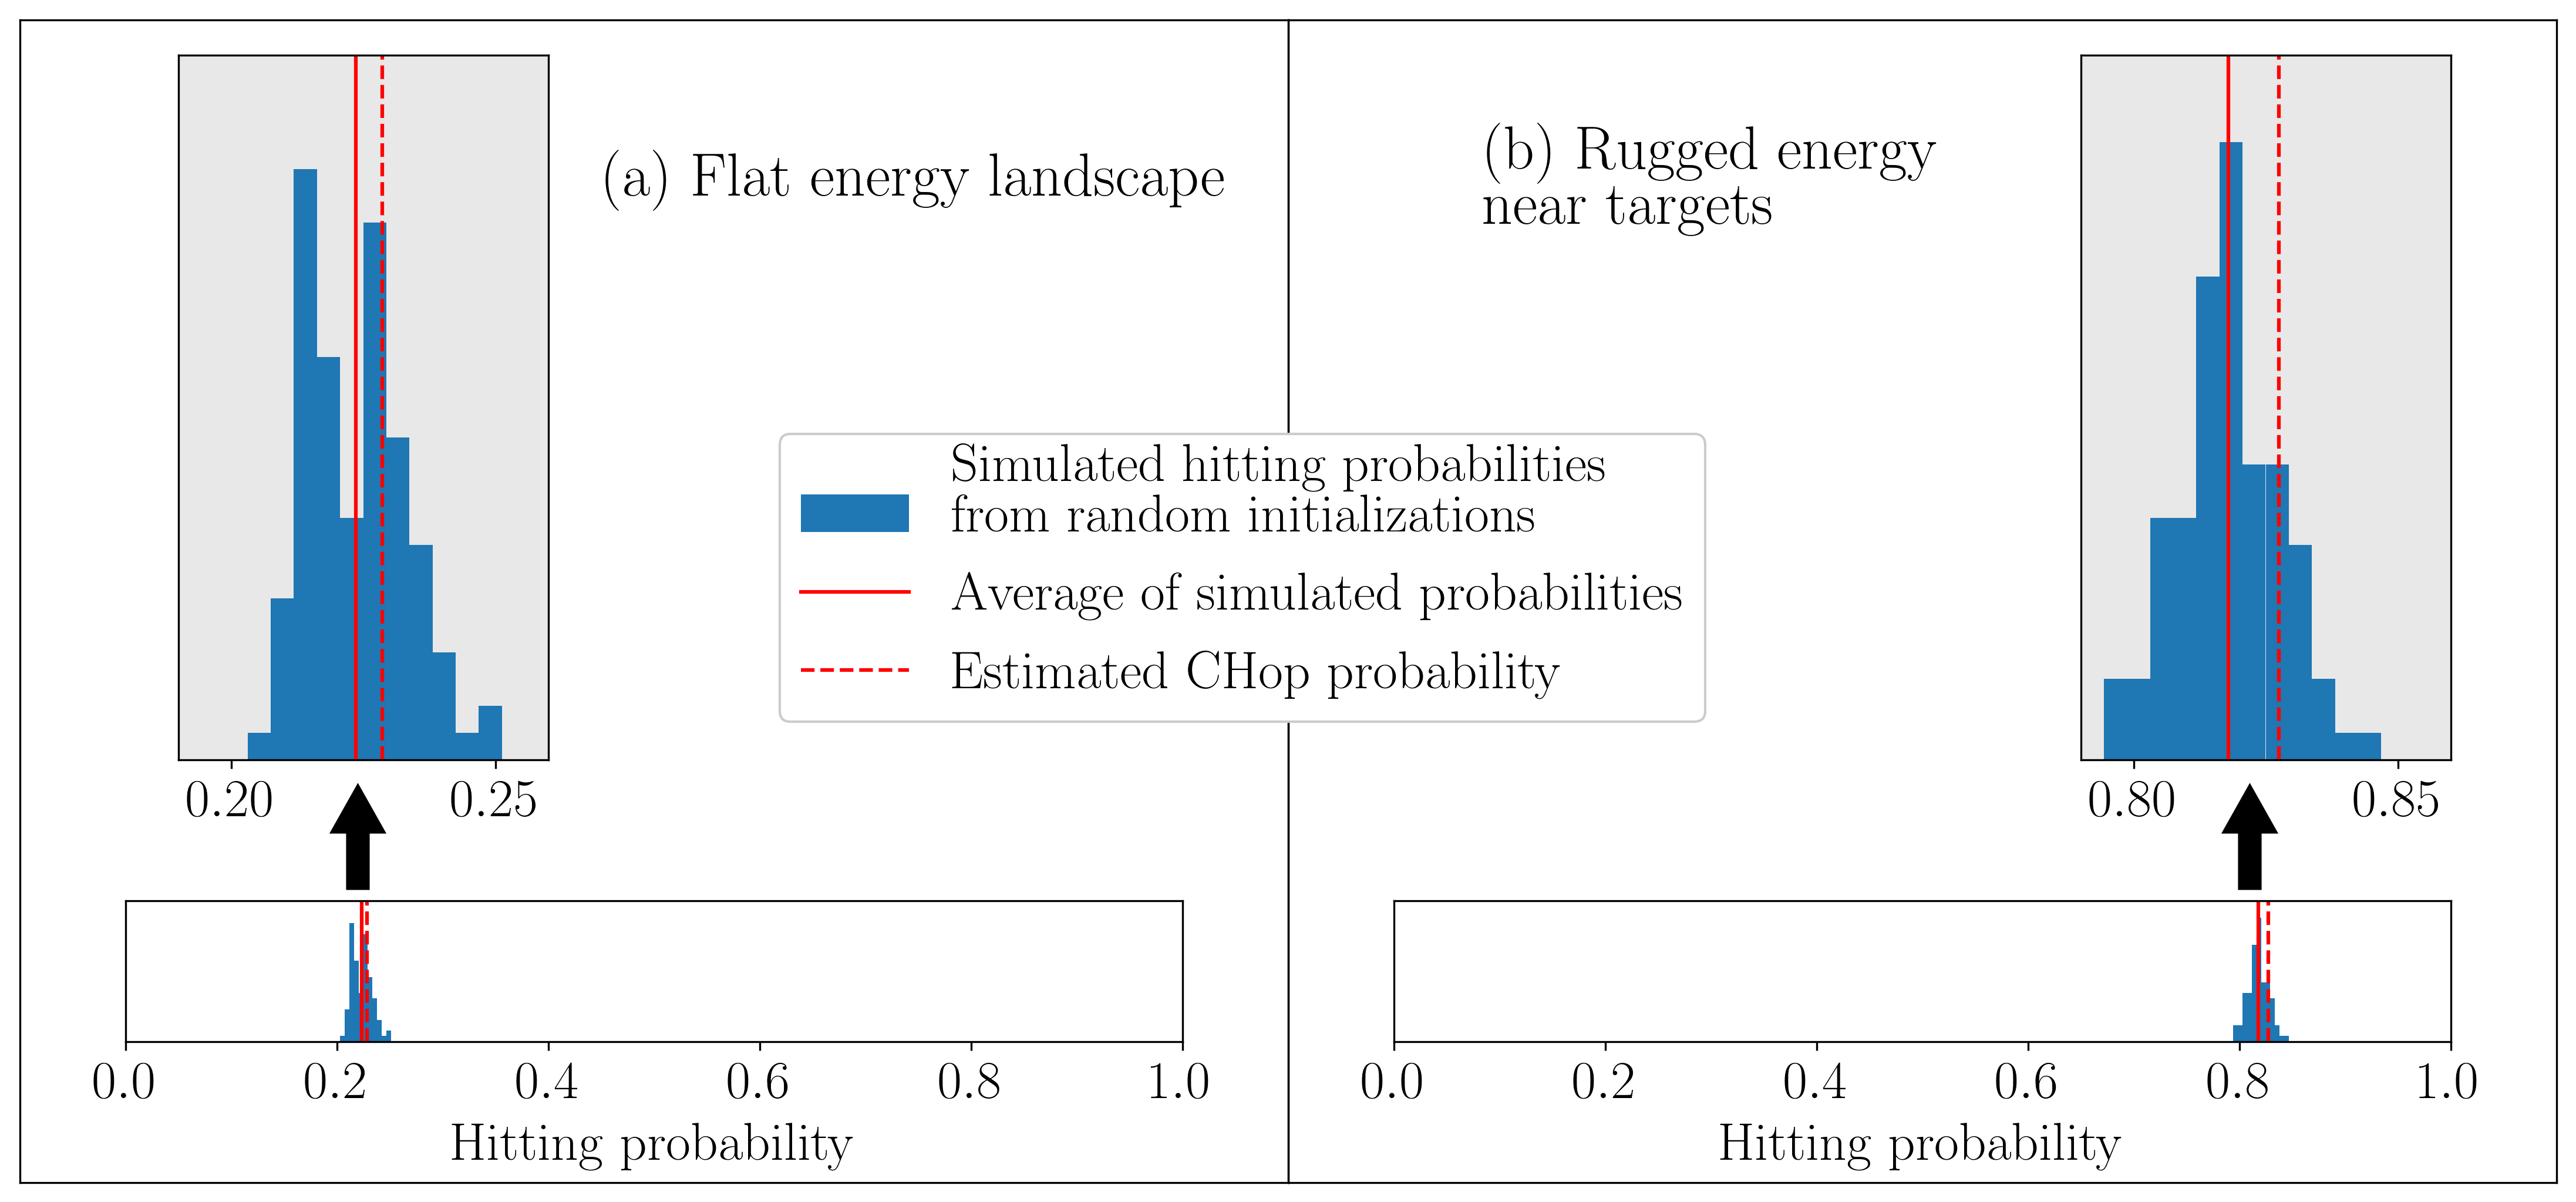
\includegraphics[width=\textwidth]{figs/results.png}
    \caption{\label{fig:results} \textbf{Simulated hitting probabilities vs. CHop probabilities}.  The CHop method accurately answers the question ``where will we go next?'' for a dynamics simulation initialized in a large, flat region of configuration space.  We start by designating two target regions, $A$ and $B$.  For any given initial condition, our task is to determine the probability that we hit $A$ first. We look at this question in the context of two different dynamics. In subfigure (a), we use the simplest possible dynamics: Brownian motion.  In subfigure (b), we consider the case that the energy landscape $U$ becomes complex and rugged near the targets of interest.  In both cases we consider 100 random initial locations which are away from either target regions.  For each initial condition, we conduct 2000 simulations to estimate the probability of hitting target $A$ first.  For both dynamics we see that the hitting probability is nearly constant for initial conditions which are away from the target regions.  Furthermore, the value of this constant is well-approximated by the CHop estimates.  These simulations show that the CHop probabilities are able to reconstruct a global property of the system, even though they completely invariant to the dynamics for the majority of configuration space.  Indeed, the CHop probabilities can be computed using only small local simulations around each target, and do not require any simulations of trajectories that cross the large, flat region between $A$ and $B$.}
\end{minipage}}
\end{figure}

The first set of experiments are ``sanity checks'' designed to show that the CHop methods works in the simplest possible case.  For these sanity checks, we work with a flat energy landscape in $\mathbb{R}^5$, where quantities of interest can be obtained in closed form.  In particular, we look at the toy model with parameters \TODOTHIS

\subsubsection{The hitting probabilities are approximately constant}

The first sanity check tests the CHop idea at its most basic level: that the large flat region of a golf-course potential features constant hitting probabilities, i.e.\ $\varepsilon$-flatness.  Theorem \ref{thm:epsilon_flat} shows that this must hold in the limiting regime of small $r_A,r_B$, but it is not obvious whether the parameters we use lie in that regime.  

In the toy model, we see that the $\varepsilon$-flatness condition indeed holds, with $\varepsilon \approx .05$.  We ran 2000 diffusion simulations at each of 100 randomly selected initial conditions in the ``flat region'' $\mathcal{B}(0, 1) \setminus (\tilde{A} \cup \tilde{B})$.  A histogram of these probabilities may be found in Figure \ref{fig:results}.  From this we see that the hitting probabilities in this region do not substantially depend upon the initial condition, all falling in the range $[0.2055, 0.2480]$.


\subsubsection{The value of this constant is well-approximated using CHop probabilities}

Our second check tests whether the CHop probabilities accurately approximate the hitting probabilities.  For this problem, the relevant CHop probabilities can be computed in closed form:
\begin{equation}
p_A = \frac{\frac{1}{r_A^{2 - \dimension} - r_{\tilde{A}}^{2 - \dimension}}}{\frac{1}{r_A^{2 - \dimension} - r_{\tilde{A}}^{2 - \dimension}} + \frac{1}{r_B^{2 - \dimension} - r_{\tilde{B}}^{2 - \dimension}}}
\end{equation}

According to this formula, the CHop probability is $.2286$.  This is in good agreement with the average hitting probability $.2236$ found by direct simulation in the previous section.


\subsubsection{CHop capacity estimation}

Finally, we check the accuracy of the capacity estimation algorithm employed by CHop.  We can get an analytical formula for the capacities in this case.  We compare these exact values with those estimated using the method outlined in Section \ref{sec:outlinecapacest}, with parameters $m = 2, n = 4, N_p = 100, N_b = 3,N_s = 1000$ and a time-step of $10^{-6}$.  We obtain the following results:

\begin{itemize}
\item $\capac{A}{\tilde{A}}=$\TODOTHIS, and our method obtained the estimate \TODOTHIS
\item $\capac{B}{\tilde{B}}=$\TODOTHIS, and our method obtained the estimate \TODOTHIS
\end{itemize}

These show good agreement between the truth and our estimates.

\subsection{Results on Nontrivial Energy Landscape}

In this section, we apply the CHop method to a model with a nontrivial energy landscape around the targets. We see that our algorithm can accurately estimate the hitting probabilities while maintaining great advantage over the direct simulations in terms of speed.

We experimented with the toy model parameters with $d = 5$ and
\begin{equation*}
x_A = \begin{pmatrix}%
0.5&0.6&0.0&0.0&0.0%
\end{pmatrix},
r_A = 0.02,
d_A = 0.05,
r_{\tilde{A}} = 0.1
\end{equation*}
for target $A$, and
\begin{equation*}
x_B = \begin{pmatrix}%
-0.7&0.0&0.0&0.0&0.0%
\end{pmatrix},
r_B = 0.04,
d_B = 0.075,
r_{\tilde{B}} = 0.15
\end{equation*}
for target $B$.  We refer the reader to Appendix \ref{sec:energy_function} for more details.

\subsubsection{The hitting probabilities are approximately constant}

We again start by testing the basic idea of CHop: we use direct simulations to test the hypothesis that the hitting probabilities are relatively flat in away from the targets.  The results can be seen in Figure \ref{fig:results}.   For every initial condition we tested, we found that the hitting probability fell in the interval $[0.7980, 0.8450]$, suggesting that the $\varepsilon$-flatness condition holds with $\varepsilon \approx .05$.



\subsubsection{The value of this constant is well-approximated using CHop probabilities}

Using the CHop capacity estimation procedure from Section \ref{sec:outlinecapacest}, we obtained an estimate of $0.8274$ for the CHop probability of this model.  This is in good agreement with the average hitting probability $.8180$ found in our direct simulations.  For the capacity estimation procedure, we used the parameters $m=2,N_p=5000,N_b=10,N_s=2000$ and a time-step of $10^{-7}$.  For the $A$ capacity we used $n=4$ and for the slightly larger $B$ region we used $n=5$.  

\subsubsection{CHop capacity estimation}

In this case it is difficult to assess the accuracy of the CHop capacity algorithm.  It is not possible to obtain exact values for the capacity.  Therefore, we cannot directly test whether our algorithm is accurately estimating the capcities.  However, as the last section showed, the CHop probabilities computed from our estimated capacities do seem to accurately reflect the true hitting probabilities.  This offers some limited evidence that the estimated capacities are also accurate.

We can also test the speed of CHop capacity estimation algorithm.  We compared the time it takes to estimate the hitting probabilities using direct simulations with the time our capacity estimation algorithm needs to estimate the capacities for all targets. Note that in order to make the direct simulations feasible for the $5$-dimensional toy model we are working on, we made our best effort to make the direct simulation fast.  We use an efficient walk-on-spheres method to simulate trajectories in the flat region,\cite{bingham1972random} JIT compilation to remove loop overhead, 24-CPU parallization, and a relatively coarse time step.  The CPU times for the direct simulations and the CHop method are shown below:

\begin{description}
\item[Direct simulation] 89177.87 seconds (3715.74 seconds on a cluster of 24 CPUs).  This quantity is the sum over the amount of time it took to run 2000 simulations for each of the 100 different initial locations, using a relatively coarse time step of $10^{-5}$.  These direct simulations are trivial to perform in parallel, assuring us that there was no significant overhead due to the parallelization.

\item[CHop speed] 1055.55 seconds on a single CPU. In doing this we employed a time step which was 100 times more accurate than the one used for direct simulation (i.e.\ a timestep of $10^{-7}$). Despite this, the CHop algorithm was three times faster on a single node than the direct method run on a cluster of 24 nodes.

\end{description}

This reflects an 85-fold acceleration.  Furthermore note that the time-consuming elements of the capacity estimation algorithm are ``embarassingly parallelizable'' and should be easy to further accelerate using parallelization.  There was no need to do so in this case because we could easily run the CHop code on our laptops.  However, larger scale problems would certainly benefit from this kind of acceleration.  

The times reported above reflect a particular choice of parameters, but we found that the accuracy of the algorithm was fairly robust to choices of $N_p, N_b$ and $N_s$.  For example, we performed another experiment with time step of $10^{-6}$, parameters of $ m = 2, n = 4, N_p = 3000, N_b = 5, N_s = 1000 $ for estimating the $A$ capacity, and parameters of $ m = 2, n = 5, N_p = 3000, N_b = 5, N_s = 1000 $ for estimating the $B$ capacity.  The result was an estimate of $0.8420$. This still agrees well with the direct simulations (indeed, there were some initial conditions for which the direct simulation hitting probability estimates agreed with this quantity almost exactly).  Using these parameters, total computation time was reduced to 119.35 seconds, reflecting a 750-fold acceleration.


%                       _           _                 
%   ___ ___  _ __   ___| |_   _ ___(_) ___  _ __  ___ 
%  / __/ _ \| '_ \ / __| | | | / __| |/ _ \| '_ \/ __|
% | (_| (_) | | | | (__| | |_| \__ \ | (_) | | | \__ \
%  \___\___/|_| |_|\___|_|\__,_|___/_|\___/|_| |_|___/
                                                    

\section{Discussion and Future Directions}\label{sec:conclusion}

Shape is function for many dynamic processes, including proteins and non-coding RNAs. Being in the right state at the right time can be difficult\cite{Levinthal1968-ov} and getting it wrong is often fatal.\cite{Luheshi2008-wd} It is vitally important that macromolecules can reliably fold to the right state, time and time again. However, more than 50 years after the demonstration that protein folding is a straightforward biophysical process \cite{Anfinsen1961-xe}, and more than 25 years after the clear formulation of the RNA folding problem \cite{Draper1992-pm}, high-quality simulation algorithms remain elusive.   

A majority of previous developments have focused on analysis of \emph{enthalpic barriers} and the properties of dynamics stuck in local minima.\cite{Christen2008-ge}  Proper understanding of these enthalpic effects can tremendously accelerate simulation.  Transition state theory\cite{Eyring1935-ur, Chandler1978-bq, Wigner1997-kk} is perhaps the foundational work in this direction. Various other methods build on top of this, including different accelerated molecular dynamics methods\cite{Perez2009-jy}(hyperdynamics\cite{Voter1997-gi}, parallel replica\cite{Voter1998-mv} and temperature-accelerated dynamics\cite{Sorensen2000-qm}), transition path sampling,\cite{Dellago1998-lb, Bolhuis2002-ws} transition interface sampling,\cite{Van_Erp2005-vw} and the more recent transition path theory.\cite{E2006-fm, E2010-sr} The accelerated molecular dynamics methods achieve the acceleration by either smoothing the energy landscape, exploring energy basins in parallel, or raising the temperature while maintaining the correct dynamics. For transition path sampling, transition interface sampling and the transition path theory, the basic idea is to providing information about the reaction rates between different states, with the transition path theory also giving us a theoretical framework and a more comprehensive picture of the actual reaction processes.

Though these advances have significantly accelerated simulation, molecular dynamics methods still spend enormous computational effort simulating trajectories across \emph{entropic barriers} to get in the vicinity of small target regions.  In many important problems, the key regions of configuration space are quite small from a combinatorial point of view.\cite{McLeish2005-dq}  This means that it may take a long time to simulate trajectories which hit those small targets -- not because of any local energetic minima, but simply because of the vastness of configuration space.  Traditional acceleration techniques are not always applicable to this problem.\cite{Baum1986-we, Wille1987-tf, Machta2009-gh} 

In this work, we offer new insight into these crucial ``small-target'' problems, from a hitting-probability perspective.  While offering less kinetic insight than direct simulation, hitting probabilities offer more kinetic understanding than purely thermodynamic analyses.  We show that hitting probability problems with small targets often feature an approximate invariance to initial conditions away from the targets.  This invariance can then be used to show invariance to the energy landscape away from the targets.  This means that the probabilities can be calculated using only local simulations around the targets.  We hope this offers some light into the broader problem of understanding the role of entropy in the kinetics of complex molecular dynamics.  We also use these insights to produce CHop, an practical algorithm to estimate hitting probabilities for small-target problems.  

Simulations suggest that CHop is highly effective for small-target problems, both in terms of accuracy and speed.  However, simulations can be deceiving.  In future work, we hope to apply CHop to real-world problems to see if novel insights can be gained using this capacity-based perspective.  

\appendix

%%%%%%%%%%%%%%%%%%%%%%%%%%%%%%%%%%%%%%%%%%%%
%%%%%%%%%%%%%%%%%%%%%%%%%%%%%%%%%%%%%%%%%%%%
%%%%%%%%%%%%%%%%%%%%%%%%%%%%%%%%%%%%%%%%%%%%
%%%%%%%%%%%%%%%%%%%%%%%%%%%%%%%%%%%%%%%%%%%%
%   __ _ _ __   __| |_  __
%  / _` | '_ \ / _` \ \/ /
% | (_| | |_) | (_| |>  < 
%  \__,_| .__/ \__,_/_/\_\
%       |_|               
%%%%%%%%%%%%%%%%%%%%%%%%%%%%%%%%%%%%%%%%%%%%
%%%%%%%%%%%%%%%%%%%%%%%%%%%%%%%%%%%%%%%%%%%%
%%%%%%%%%%%%%%%%%%%%%%%%%%%%%%%%%%%%%%%%%%%%
%%%%%%%%%%%%%%%%%%%%%%%%%%%%%%%%%%%%%%%%%%%%

\appendix

%     _    ____  ____  _____ _   _ ____ _____  __     _    
%    / \  |  _ \|  _ \| ____| \ | |  _ \_ _\ \/ /    / \   
%   / _ \ | |_) | |_) |  _| |  \| | | | | | \  /    / _ \  
%  / ___ \|  __/|  __/| |___| |\  | |_| | | /  \   / ___ \ 
% /_/   \_\_|   |_|   |_____|_| \_|____/___/_/\_\ /_/   \_\
                                                         


\section{Stationary Reversible Diffusion Processes}\label{sec:reversible_diffusion}

In this section, we set notation and review some properties of stochastic differential equations.   Let $\{X_t\}_{t \geqslant 0}$ denote a stationary reversible diffusion process trapped in 
$\Omega \subset \mathbbm{R}^\dimension$ by reflecting boundaries, with continuous invariant density $e^{-U}$, satisfying 
%
\[ \mathrm{d} X_t = b (X_t) \mathrm{d} t + \sigma (X_t) \mathrm{d} W_t \]
%
where $W$ is a $d$-dimensional Brownian motion and $b (\cdot) : \mathbbm{R}^\dimension \rightarrow \mathbbm{R}^\dimension,\sigma
(\cdot) : \mathbbm{R}^\dimension \rightarrow \mathbbm{R}^{\dimension \times d}$ are differentiable.  If no boundaries are desired, we can take $\Omega= \mathbb{R}^\dimension$.  Recall that $b$ is entirely determined by $\sigma,U$ and the requirement that the process is stationary and reversible; indeed, per Proposition 4.5 of Pavliotis\cite{Pavliotis2016-xn} we have that $b_i(x)=\frac{1}{2} \sum_j \partial a_{ij}(x)/\partial x_j + \sum_j a_{ij}(x) \partial U(x)/\partial x_j$ where $a=\sigma\sigma^T$.  We refer to Bovier\cite{Bovier2016-ez} and Pavliotis\cite{Pavliotis2016-xn} for a useful exposition on these kinds of processes.

This paper's main results arise from consideration of three related objects induced by this diffusion: the Dirichlet form, the capacity, and the Dirichlet problem.  

\begin{definition}
The \textbf{Dirichlet form} of $X$ is given
by
\[ \mathcal{E} (f, g) = \frac{1}{2} \int_\Omega (\sigma(x) \nabla f (x))^T 
 (\sigma(x) \nabla g (x)) e^{- U (x)} \mathrm{d} x \]
\end{definition}

This form induces a ``capacity'' on pairs of nested sets:

\begin{definition}
Let $A \subset \tilde{A} \subset \Omega$ be non-empty. Assume we have an
open set $D \subset \Omega$ for which $\partial D = \partial A \cup \partial
\tilde{A}$ and smooth. The \textbf{capacity} $\ensuremath{\operatorname{cap}} (A, \tilde{A})$ is defined as
%
\[ \ensuremath{\operatorname{cap}} (A, \tilde{A}) = \inf_{f \in
\mathcal{H_{A, \tilde{A}}}} \mathcal{E} (f, f) \]
%
where $\mathcal{H}_{A, \tilde{A}}$ is the space of functions $f$ such that
\begin{enumerate}
\item $f \in H^1$, where $H^1$ is the Soblev space of weakly
differentiable functions

\item $\mathcal{E} (f, f) < \infty$

\item $f \geqslant 1$ on $\partial A$ and $f \leqslant 0$ on $\partial
\tilde{A}$
\end{enumerate}

\end{definition}

The capacity is intimately connected with a partial differential equation known as the Dirichlet problem:

\begin{definition}
Let $A, B \subset \Omega$ be non-empty and disjoint.  The \textbf{Dirichlet problem} for $A,B$ with respect to the diffusion $X$ is defined as the partial
differential equation
\[ 0 = \sum_{i = 1}^\dimension b_i (x) \frac{\partial f
(x)}{\partial x_i} + \frac{1}{2} \sum_{i = 1}^\dimension \sum_{j = 1}^\dimension a_{ij} (x)
\frac{\partial^2 f (x)}{\partial x_i \partial x_j} \]
where $a(x)=\sigma(x)\sigma(x)^T$, with boundary conditions
\begin{eqnarray*}
h (x) & = & 1, x \in A\\
h (x) & = & 0, x \in B
\end{eqnarray*}
As long as there is some set $D \subset \Omega$ for which $\partial D = \partial A \cup \partial B$, this problem has a unique solution which we will denote $h_{A,B}$.
\end{definition}

The connection between the capacity and the Dirichlet problem is given by the following, proved in Theorem 7.33 of Bovier:\cite{Bovier2016-ez}

\begin{proposition}\label{prop:capacitydirichlet}
If $\mathcal{H}_{A, \tilde{A}} \neq \varnothing$, then
\[
\capac{A}{\tilde{A}} = \mathcal{E} (h_{A,\tilde{A}^c}, h_{A, \tilde{A}^c})
\]
\end{proposition}

At first glance, it is unclear why any of these objects are relevant to the study of the diffusion $X$.  The answer comes in the form of the celebrated {\itshape{Dirichlet Principle}}, which states that the solution to the Dirichlet problem carries the probabilistic interpretation 
\[ h_{A, B} (x) =\mathbbm{P} (X_{\tau_{A \cup B}} \in A|X_0 = x) \]
where $\tau_S \triangleq \inf \{ t \geqslant 0 : X_t \in S \}$.  That is, $h_{A, B} (x)$ is the probability for $X$ to hit $A$ first before hitting $B$ if we start the process at $x$.  The Dirichlet principle is the key that connects hitting probabilities to the capacity and enables the main results of this work.


%     _    ____  ____  _____ _   _ ____ _____  __  ____  
%    / \  |  _ \|  _ \| ____| \ | |  _ \_ _\ \/ / | __ ) 
%   / _ \ | |_) | |_) |  _| |  \| | | | | | \  /  |  _ \ 
%  / ___ \|  __/|  __/| |___| |\  | |_| | | /  \  | |_) |
% /_/   \_\_|   |_|   |_____|_| \_|____/___/_/\_\ |____/ 
                                                       


\section{Proof of the Main Theorem}\label{sec:proof_thm}

Assume $X$ is a reversible stationary diffusion on $\Omega$ governed by Equation (\ref{equ:general_sde}).  Let $A\subset\tilde A\subset\Omega,B\subset\tilde B\subset\Omega$.  Let $\tilde A,\tilde B$ be disjoint and $\Omega \backslash (\tilde A \cup \tilde B)$ $\varepsilon$-flat for the hitting probabilities $h_{A,B}(x)$.  Let us assume the set boundaries are all smooth.  

Under these conditions, we will show we can use local capacities to get good approximations for $h_{A,B}(x)$ when $x\notin \tilde A,\tilde B$.  To do so, our key idea is to uncover upper and lower bounds on the value of the Dirichlet form applied to this function, $\mathcal{E}(h_{A,B},h_{A,B})$.  We will see that these bounds can be understood in terms of capacities, and the resulting inequalities will then yield our main result in the form of Theorem \ref{thm:main_thm}.

\begin{lemma}  The Dirichlet form of $h_{A,B}$ can be upper-bounded in terms of the capacities:
\[ \mathcal{E} (h_{A,B}, h_{A,B}) \leqslant \frac{\tmop{cap} (A, \tilde{A}) \tmop{cap} (B,
\tilde{B})}{\tmop{cap} (A, \tilde{A}) + \tmop{cap} (B, \tilde{B})} \]
\end{lemma}
\begin{proof}
Per Proposition \ref{prop:capacitydirichlet} and the Dirichlet principle, we have that 
%
\[
\mathcal{E} (h_{A,B}, h_{A,B}) = \capac{A}{B^c} \leq \mathcal{E} (u,u)
\]
%
for any $u\in \mathcal{H}_{A, B^c}$.  Thus, to prove an upper bound it suffices to find functions $u$ for which $u\in \mathcal{H}_{A, B^c}$ and we can calculate $\mathcal{E}(u,u)$.  To this end, consider
%
\[
u_c (x) \triangleq \left\{ \begin{array}{ll}
(1 - c) h_{A, \widetilde{A}^c} (x) + c & \tmop{if} x \in \tilde{A}\\
c (1 - h_{B, \widetilde{B}^c} (x)) & \tmop{if} x \in \tilde{B}\\
c & \tmop{otherwise}
\end{array} \right. 
\]
%
These functions are well-suited to giving us upper bounds on $\mathcal{E} (h_{A,B}, h_{A,B})$.  Indeed:
\begin{itemize}
\item $u_c \in \mathcal{H}_{A, B^c}$.  Indeed, $u_c$ takes a constant value $c$ outside of $\tilde A,\tilde B$, drops smoothly to in $\tilde B$ to achieve 0 on $\partial B$, and rises smoothly in $\tilde A$ to achieve 1 on $\partial \tilde A$.  Thus, since we have assumed the boundaries of $\tilde A,\tilde B$ are smooth, $u_c \in \mathcal H_{A,B^c}$.  
\item $\mathcal{E}(u_c,u_c)$ can be calculated by applying Proposition \ref{prop:capacitydirichlet} twice, yielding $\mathcal{E}(u_c,u_c) = (1 - c)^2 \tmop{cap} (A, \tilde{A}) + c^2 \tmop{cap} (B, \tilde{B})$.
\end{itemize}
Thus the $u_c$ functions give us a practical way to calculate upper bounds: 
\[
\mathcal{E} (h_{A,B}, h_{A,B})\leq (1 - c)^2 \tmop{cap} (A, \tilde{A}) + c^2 \tmop{cap} (B, \tilde{B})
\]
This inequality holds for any value of $c$.  To get the best bound, we can take derivatives to minimize the right hand side with respect to $c$.  The result is 
\[
c^* = \frac{\capac{A}{\tilde A}}{\capac{A}{\tilde A}+\capac{B}{\tilde B}}
\]
Plugging this into the previous equation, we obtain our final result.
\end{proof}

%%%%%%%%%%%
%%%%%%%%%%%

\begin{lemma}  Let $m = \frac{1}{2} (\sup_{x \notin \tilde A,\tilde B} h_{A,B} (x) + \inf_{x \notin \tilde A,\tilde B} (h_{A,B} (x)))$.  The Dirichlet form of $h_{A,B}$ can be lower-bounded in terms of $m$ and the capacities:
\[\mathcal{E} (h_{A,B}, h_{A,B}) \geq  
   \left( 1 - m - \frac{\varepsilon}{2} \right)^2 \tmop{cap} (A,\tilde{A}) \indicatorf{m\leq 1-\frac{\varepsilon}{2}} + 
   \left( m- \frac{\varepsilon}{2} \right)^2 \tmop{cap} (B, \tilde{B})\indicatorf{m\geq \frac{\varepsilon}{2}} 
\]
\end{lemma}
\begin{proof}
Recall that $\mathcal{E} (h_{A,B}, h_{A,B})$ can be expressed as an integral over $\Omega$.  We decompose this into three integrals: one over $\tilde A$, one over $\Omega \backslash \tilde A,\tilde B$, and one over $\tilde B$.  
\[
\mathcal{E} (h_{A,B}, h_{A,B}) = \int_{\tilde A} \Vert \sigma \nabla h_{A,B}\Vert^2 dx
                                 + \int_{\tilde B} \Vert \sigma \nabla h_{A,B}\Vert^2 dx
                                 + \int_{\Omega \backslash \tilde A,\tilde B} \Vert \sigma \nabla h_{A,B}\Vert^2 dx
\]
Since the integrand is always positive, we can get a lower bound by simply ignoring the integral over $\Omega \backslash \tilde A,\tilde B$ and focusing on the integrals over $\tilde A,\tilde B$.  The $\tilde A,\tilde B$ integrals can be lower-bounded using capacities.  

For example, let us focus on the $A$ case.  There are two different possibilities we must consider:
\begin{itemize}
\item If $m>1-\varepsilon/2$ we will simply note that the integral over the $\tilde A$ region is nonnegative.  
\item If $m\leq 1-\varepsilon/2$, then we define
    \[
    u_A (x) \triangleq \frac{h_{A,B} (x) - m - \frac{\varepsilon}{2}}{1 - m - \frac{\varepsilon}{2}}
    \]
    Note that $u_A \in \mathcal H_{A,\tilde A}$.  Indeed, $h_{A,B}(x)=1$ for $x \in \partial A$ and the $\varepsilon$-flatness condition shows that $h_{A,B}(x) \leq m + \frac {1}{2}$ for $x \in \partial \tilde A$.  Thus, applying the definition of the capacity, we see that $\mathcal{E}(u_A,u_A) \geq \capac{A}{\tilde A}$.  Thus we see that
    %
    \begin{align*}
    \int_{\tilde A} \Vert \sigma \nabla h_{A,B}\Vert^2 dx &= \left(1 - m - \frac{\varepsilon}{2}\right)^2 \int_{\tilde A} \Vert \sigma \nabla u_{A}\Vert^2 dx\\
         &\geq \left(1 - m - \frac{\varepsilon}{2}\right)^2 \capac{A}{\tilde A}
    \end{align*}
\end{itemize}
Putting these together, we obtain
\[
\int_{\tilde A} \Vert \sigma \nabla h_{A,B}\Vert^2 dx \geq \left(1 - m - \frac{\varepsilon}{2}\right)^2 \capac{A}{\tilde A}\indicatorf{m\leq 1-\frac{\varepsilon}{2}}
\]
Applying the same ideas to the integral over $\tilde B$, we obtain our result.
\end{proof}

%%%%%%%%%%%
%%%%%%%%%%%


\begin{thm*}  The hitting probabilities can be well-approximated by the capacities:
\[ \sup_{x \notin \tilde A,\tilde B} \left| h_{A,B} (x) - \frac{\ensuremath{\operatorname{cap}} (A,
\tilde{A})}{\ensuremath{\operatorname{cap}} (A, \tilde{A})
+\ensuremath{\operatorname{cap}} (B, \tilde{B})} \right| \leqslant \varepsilon + \sqrt{\varepsilon/2} \]
\end{thm*}

\begin{proof}
\global\long\def\capA{\kappa_A}
\global\long\def\capB{\kappa_B}

To simplify notation, let $\capA=\capac{A}{\tilde A}$ and $\capB=\capac{B}{\tilde B}$.  Applying the previous two lemmas together, we obtain the inequality
\[
\frac{\capA \capB}{\capA +\capB}
\geq \mathcal{E}(h_{A,B},h_{A,B}) \geq
\left( 1 - m - \frac{\varepsilon}{2} \right)^2 \capA \indicatorf{m\leq 1-\frac{\varepsilon}{2}} + 
   \left( m- \frac{\varepsilon}{2} \right)^2 \capB \indicatorf{m\geq \frac{\varepsilon}{2}} 
\]
where $m = \frac{1}{2} (\sup_{x \notin \tilde A,\tilde B} h_{A,B} (x) + \inf_{x \notin \tilde A,\tilde B} (h_{A,B} (x)))$.  In analyzing this inequality, there are three possibilities to consider.  
\begin{itemize}
    \item If $m \in (\epsilon/2,1-\epsilon/2)$, the quadratic formula yields
    \begin{eqnarray*}
    m & \geqslant & \frac{\capA}{\capA + \capB} + \frac{
    \frac{\varepsilon}{2}(\capB - \capA) - 
    \sqrt{\capA \capB \varepsilon( 2 - \varepsilon)}}{\capA+\capB}\\
    m & \leqslant & \frac{\capA}{\capA + \capB} + \frac{
    \frac{\varepsilon}{2}(\capB - \capA) +
    \sqrt{\capA \capB \varepsilon( 2 - \varepsilon)}}{\capA+\capB}
    \end{eqnarray*}
    Applying $\left|\frac{\capB - \capA}{\capA + \capB}\right| \leq 1$ and the fact that the geometric mean $\sqrt{\capA \capB}$ never exceeds the arithmetic mean $(\capA+\capB) / 2$, it follows that
    \[
    \left|m -  \frac{\capA}{\capA + \capB}\right| \leq \frac{\epsilon +\sqrt{\epsilon (2-\epsilon)}}{2}
    \]
    Applying the fact that $m$ was designed so that $|h_{A,B}(x) - m| <\varepsilon/2$ for all $x \notin \tilde A,\tilde B$, we obtain
    \[
    \left|h_{A,B}(x) -  \frac{\capA}{\capA + \capB}\right| \leq \frac{2\epsilon +\sqrt{\epsilon (2-\epsilon)}}{2}
    \]

    \item If $m<\varepsilon/2$, our equations become 
    \[
    \frac{\cancel{\capA} \capB}{\capA +\capB}
    \geq
    \left( 1-m- \frac{\varepsilon}{2} \right)^2 \cancel{\capA} 
    \]
    Our assumption that $m \leq \varepsilon/2$ indicates that $(1- m- \varepsilon/2)^2 \geq (1-\varepsilon)^2$, thus in fact we have 
    \[
    \frac{\capB}{\capA +\capB}
    \geq
    \left( 1- \varepsilon \right)^2  = 1 + \varepsilon^2 - 2\varepsilon
    \]
    which means that $\capA/(\capA +\capB)
    \leq
    2\varepsilon - \varepsilon^2 \leq 2\varepsilon$.  
    Thus we assumed $m\in[0,\varepsilon/2]$ and showed that $\capA/(\capA+\capB)\in[0,2\varepsilon-\varepsilon^2]$, so it follows that 
    \[
    \left|m -  \frac{\capA}{\capA + \capB}\right| \leq 2\varepsilon -\varepsilon^2
    \]
    and so for any $x\notin \tilde A,\tilde B$, we have 
    \[
    \left|h_{A,B}(x) -  \frac{\capA}{\capA + \capB}\right| \leq 2.5\varepsilon -\varepsilon^2
    \]
    
    \item If $m>1-\varepsilon/2$, the same bound can be achieved by arguments which are symmetric to those employed in $m<\varepsilon/2$:
    \[
    \left|h_{A,B}(x) -  \frac{\capA}{\capA + \capB}\right| \leq 2.5\varepsilon -\varepsilon^2
    \]
\end{itemize}
Our final result is found by noting that all these bounds are upper-bounded by $\varepsilon + \sqrt{\varepsilon/2}$.
\end{proof}

%     _    ____  ____  _____ _   _ ____ _____  __   ____ 
%    / \  |  _ \|  _ \| ____| \ | |  _ \_ _\ \/ /  / ___|
%   / _ \ | |_) | |_) |  _| |  \| | | | | | \  /  | |    
%  / ___ \|  __/|  __/| |___| |\  | |_| | | /  \  | |___ 
% /_/   \_\_|   |_|   |_____|_| \_|____/___/_/\_\  \____|
           

\section{Proof of the $\varepsilon$-flatness of the Toy Model}\label{sec:proof_epsilon_flat}

Consider the setup of the Toy Model described in Section \ref{sec:toy_model}.  A stationary reversible diffusion $X$ is trapped inside the unit $\dimension$-dimensional ball.  We are interested to know which target $X$ will hit first: $A=\bb{x_A,r_A}$ or $B=\bb{x_B,r_B}$.  The function $h_{A,B}(x)$ indicates the probability we will hit $A$ first if $X_0=x$.  We will be particularly interested in the csae where $X_0$ is outside of $\tilde A=\bb{x_A,d_A},\tilde B=\bb{x_A,d_B}$.  Also recall that in the toy example the diffusion behaves as a Brownian motion outside of $\dot A=\bb{x_A,d_A},\dot B=\bb{x_B,d_B}$.  

It turns out that by taking the $\dimension$ is sufficiently high or $d_A,d_B$ are sufficiently small, we can make the hitting probabilities arbitrarily close to constant in the region away from $\tilde A,\tilde B$:

\begin{thm*}  For any fixed value of the ambient dimension $\dimension \geq 3$ and any $r_{\tilde{A}}, r_{\tilde{B}}, \varepsilon > 0$, there exists a constant $c=c(\dimension, r_{\tilde{A}}, r_{\tilde{B}}, \varepsilon)$ such that if $d_{A}, d_{B} < c$ then $\bb {0, 1} / (\tilde{A} \cup \tilde{B})$ is $\varepsilon$-flat for the function $h_{A,B}(x)$.  Likewise for any fixed value of $d_{A}, r_{\tilde{A}}, d_{B}, r_{\tilde{B}}, \varepsilon>0$, there exists a constant $c=c(d_{A}, r_{\tilde{A}}, d_{B}, r_{\tilde{B}}, \varepsilon)$ such that if $\dimension \geq c$ then $\bb {0, 1} / (\tilde{A} \cup \tilde{B})$ is $\varepsilon$-flat for the function $h_{A,B}(x)$.
\end{thm*}

\begin{proof}
Let us assume $X_0 \notin \tilde A,\tilde B$.  There are essentially two things that must be proved:
\begin{enumerate}
\item The process $X$ converges to its stationary distribution fairly quickly.  This is supported by Lemma \ref{lem:uniform_ergodicity}.  Since $h_{A,B}(x) \in [0,1]$, this Lemma gives that
%
\[
|\mathbb{E}[h_{A,B}(M_t)-h_{A,B}(Z)]| \leq 2^2/4t =1/t
\]
%
where $Z$ is distributed according to the uniform distribution on $\Omega$ and $M$ is a Brownian motion trapped in $\Omega$ by normally reflecting boundaries.  

To connect this result on $M$ to our object of interest $h_{A,B}$, note that without loss of generality we may assume $X,M$ are on the same probability space and $M_t=X_t$ for $t<\tilde\tau \triangleq \inf \{t:\ X_t \in \partial \dot A \cup \partial \dot B\}$.  Moreover, noting that $\tilde\tau\wedge t$ is a stopping time and applying the Strong Markov property, we observe that 
%
\[
h_{A,B}(x) = \mathbb{E} [\indicatorf{X_{t\wedge\tilde\tau} \in \partial A}] 
        = \mathbb{E} [\mathbb{E}[\indicatorf{X_{t\wedge\tilde\tau} \in \partial A} | X_{t\wedge\tilde\tau}]]
        = \mathbb{E} [h_{A,B}(X_{t\wedge\tilde\tau})] = \mathbb{E} [h_{A,B}(M_{t\wedge\tilde\tau})]
\]
%
Thus
\begin{align*}
|h_{A,B}(x) - \mathbb{E}[h_{A,B}(Z)]| &= |\mathbb{E} [h_{A,B}(M_{t\wedge\tilde\tau})] - \mathbb{E}[h_{A,B}(Z)]|\\
&\leq |\mathbb{E} [h_{A,B}(M_{t\wedge\tilde\tau})] - h_{A,B}(M_t)]| + |\mathbb{E} [h_{A,B}(M_{t}) - h_{A,B}(Z)]|\\
&\leq \mathbb{P}(\tilde \tau \leq t) + 1/t
\end{align*}
%

\item The hitting time $\tilde \tau$ is generally long.  This is supported by Lemma \ref{lem:longtime}.  This says that if $X_0 \not\in\tilde{A} \cup \tilde{B}$ we can ensure
%
\[
\mathbbm{P} \left( \tilde{\tau} < \frac{8}{\varepsilon} \right) < \frac{\varepsilon}{4} 
\]
%
for arbitrarily small $\varepsilon$ by taking $\dimension$ sufficiently high or $d_A,d_B$ sufficiently small.
\end{enumerate}
Putting these two results together at $t=8/\varepsilon$ we obtain that we can make $|h_{A,B}(x) - \mathbb{E}[h_{A,B}(Z)]| \leq \varepsilon / 4 + \varepsilon/8 \leq \varepsilon$ for arbitrarily small $\varepsilon$ by taking $\dimension$ sufficiently high or $d_A,d_B$ sufficiently small.
\end{proof}

%%%%%%%%%%%%%%%%%%%%%%
%%%%%%%%%%%%%%%%%%%%%%

\begin{lemma}
\label{lem:uniform_ergodicity}(Uniform ergodicity) Let $\Omega\subset\mathbbm{R}^d$ be a convex set with diameter $\xi$ and let $M$ denote a Brownian motion trapped by reflecting boundaries inside $\Omega$.  The distribution of $M_t$ converges uniformly to the uniform distribution:
%
\[ 
\sup_{f:\ \Omega\rightarrow [0,1]} | \mathbb{E}[f(M_t) - f(Z)|M_0=x]| \leq \xi^2/4t \qquad \forall x\in \Omega, t>0
\]
%
where $Z$ is uniformly distributed on $\Omega$.
\end{lemma}
\begin{proof}
Let $F_\xi(t)$ denote the survival function for the first exit time of a one-dimensional Brownian motion from the intervals $[-\xi,\xi]$ when initialized at the origin.  Per Loper,\cite{Loper2018} 
\[
\sup_{f:\ \Omega\rightarrow [0,1]} | \mathbb{E}[f(M_t) - f(Z)|M_0=x]| \leq F_\xi(4t)
\]
It is well-known that this one-dimensional first-exit time is characterized by an expected value of $\xi^2$.  Thus, applying the Markov inequality, it follows that $F_\xi(t) \leq \xi^2 / t$ and so $F_\xi(4t) \leq \xi^2 / 4t$. 
\end{proof}

\begin{lemma}
\label{lem:longtime}Define $\tilde{\tau}_X = \inf \{ t : X_t \in \mathcal{B}
(x_A, d_A) \cup \mathcal{B} (x_B, d_B) \}$. For any fixed value of $d
\geqslant 3$ and $r_{\tilde{A}}, r_{\tilde{B}}, \varepsilon > 0$, there
exists a $c = c (d, r_{\tilde{A}}, r_{\tilde{B}}, \varepsilon)$ such that if
$d_A, d_B < c$, then
\[ \mathbbm{P} \left( \tilde{\tau}_X < \frac{8}{\varepsilon} |X_0 \not\in
\tilde{A} \cup \tilde{B} \right) < \frac{\varepsilon}{4} \]
Likewise, for any fixed value of $d_A, r_{\tilde{A}}, d_B, r_{\tilde{B}},
\varepsilon > 0$, there exists a $c = c (d_A, r_{\tilde{A}}, d_B,
r_{\tilde{B}}, \varepsilon)$, such that if the dimension $d \geqslant c$
then the same holds.
\end{lemma}

\noindent\textbf{Proof\ }First, observe that, for a given $t$,
\begin{eqnarray*}
\mathbbm{P} (\tilde{\tau}_X < t|X_0 \nin \tilde{A} \cup \tilde{B}) & = &
\mathbbm{P} (X_{\tilde{\tau}_X} \in \mathcal{B} (x_A, d_A) |X_0 \nin
\tilde{A} \cup \tilde{B}) \mathbbm{P} (\tilde{\tau}_X < t|X_{\tilde{\tau}_X}
\in \mathcal{B} (x_A, d_A), X_0 \nin \tilde{A} \cup \tilde{B})\\
& + & \mathbbm{P} (X_{\tilde{\tau}_X} \in \mathcal{B} (x_B, d_B) |X_0 \nin
\tilde{A} \cup \tilde{B}) \mathbbm{P} (\tilde{\tau}_X < t|X_{\tilde{\tau}_X}
\in \mathcal{B} (x_B, d_B), X_0 \nin \tilde{A} \cup \tilde{B})
\end{eqnarray*}
If we can establish
\begin{eqnarray*}
\mathbbm{P} \left( \tilde{\tau}_X < \frac{8}{\varepsilon}
|X_{\tilde{\tau}_X} \in \mathcal{B} (x_A, d_A), X_0 \nin \tilde{A} \cup
\tilde{B} \right) & < & \frac{\varepsilon}{4}\\
\mathbbm{P} \left( \tilde{\tau}_X < \frac{8}{\varepsilon}
|X_{\tilde{\tau}_X} \in \mathcal{B} (x_B, d_B), X_0 \nin \tilde{A} \cup
\tilde{B} \right) & < & \frac{\varepsilon}{4}
\end{eqnarray*}
Then we have proved the original result. The proofs for these two inequalities
are exactly the same. In what follows, we are going to prove
\[ \mathbbm{P} \left( \tilde{\tau}_X < \frac{8}{\varepsilon}
|X_{\tilde{\tau}_X} \in \mathcal{B} (x_A, d_A), X_0 \nin \tilde{A} \cup
\tilde{B} \right) < \frac{\varepsilon}{4} \]


Intuitively, this inequality is saying that, given we start at a point outside
$\tilde{A}, \tilde{B}$ and hit $\mathcal{B} (x_A, d_A)$ before hitting
$\mathcal{B} (x_B, d_B)$, the probability for the hitting time to be small is
small. To prove this, we pick an additional $\tilde{d}_A \in (d_A,
r_{\tilde{A}})$, and consider the trajectories of $X_t$ which start at $X_0$
and hit $\mathcal{B} (x_A, d_A)$ before hitting $\mathcal{B} (x_B, d_B)$. In
order for $X_t $to hit $\mathcal{B} (x_A, d_A)$, it has to hit $\mathcal{B}
(x_A, \tilde{d}_A)$ first. Once it hits $\mathcal{B} (x_A, \tilde{d}_A)$,
there are two possibilities: either it continues to hit $\mathcal{B} (x_A,
d_A)$, or it comes out of $\mathcal{B} (x_A, r_{\tilde{A}})$. When $d_A$
becomes small or the dimension $d$ becomes large, the probability for the
process to hit $\mathcal{B} (x_A, d_A)$ before coming out of $\mathcal{B}
(x_A, r_{\tilde{A}})$ is going to zero. Therefore it would take the process a
lot of attempts before finally hitting $\mathcal{B} (x_A, d_A)$. Each failed
attempt is associated with a certain amount of hitting time. Because of the
large number of failed attempts, the accumulated hitting time would be long
with high probability.

Formally, we are going to look at the behaviour of $X_t$ in $\mathcal{B} (x_A,
r_{\tilde{A}}) / \mathcal{B} (x_A, d_A)$ when we start on a point $x \in
\partial \mathcal{B} (x_A, \tilde{d}_A)$. Define the hitting time
\[ T = \inf \{ t : X_t \in \mathcal{B} (x_A, d_A) \cup \mathcal{B} (x_A,
r_{\tilde{A}})^c \} \]
We care about two conditional distributions: $T| | X_T - x_A | = d_A$ and $T|
| X_T - x_A | = r_{\tilde{A}}$. Note that because of symmetry, the starting
point $x$ won't affect these two distributions, as long as it's on $\partial
\mathcal{B} (x_A, \tilde{d}_A)$. It's easy to see that, if we have a sequence
of random variables
\[ T^{\tmop{out}}_1, \cdots, T^{\tmop{out}}_n, \cdots \sim T| | X_T - x_A | =
r_{\tilde{A}} \]
a random variable
\[ T^{\tmop{in}} \sim T| | X_T - x_A | = d_A \]
and a random variable
\[ N \sim \tmop{Geometric} (p), p =\mathbbm{P} (| X_T - x_A | = d_A | | X_0 -
x_A | = \tilde{d}_A) = \frac{\tilde{d}_A^{2 - d} - r_{\tilde{A}}^{2 -
d}}{d_A^{2 - d} - r_{\tilde{A}}^{2 - d}} \]
all independent of each other, $\forall t > 0$, we have
\[ \mathbbm{P} (\tilde{\tau}_X < t|X_{\tilde{\tau}_X} \in \mathcal{B} (x_A,
d_A), X_0 \nin \tilde{A} \cup \tilde{B}) \leqslant \mathbbm{P} \left(
\sum_{n = 0}^N T_n^{\tmop{out}} + T^{\tmop{in}} < t \right) \]
So we only need to establish bounds for $\mathbbm{P} \left( \sum_{n = 0}^N
T_n^{\tmop{out}} + T^{\tmop{in}} < t \right)$. For this, we note that,
$\forall s > 0$,
\begin{eqnarray*}
&  & \mathbbm{E} \left[ e^{- s \left[ \sum_{n = 0}^N T_n^{\tmop{out}} +
T^{\tmop{in}} \right]} \right]\\
& = & \mathbbm{E} \left[ e^{- sT^{\tmop{in}}} \prod_{n = 0}^N e^{-
sT_n^{\tmop{out}}} \right]\\
& = & \mathbbm{E} [e^{- sT^{\tmop{in}}}] \mathbbm{E} [(\mathbbm{E} [e^{-
sT^{\tmop{out}}}])^N]\\
& = & \mathbbm{E} [e^{- sT^{\tmop{in}}}] \sum_{k = 0}^{+ \infty} p ((1 - p)
\mathbbm{E} [e^{- sT^{\tmop{out}}}]^{})^k\\
& = & \frac{p\mathbbm{E} [e^{- sT^{\tmop{in}}}]}{1 - (1 - p) \mathbbm{E}
[e^{- sT^{\tmop{out}}}]}
\end{eqnarray*}
where $T^{\tmop{out}} \sim T| | X_T - x_A | = r_{\tilde{A}}$.

If we can bound $\mathbbm{E} \left[ e^{- s \left[ \sum_{n = 0}^N
T_n^{\tmop{out}} + T^{\tmop{in}} \right]} \right]$, we would then be able to
bound $\mathbbm{P} \left( \sum_{n = 0}^N T_n^{\tmop{out}} + T^{\tmop{in}} < t
\right)$. To bound $\mathbbm{E} \left[ e^{- s \left[ \sum_{n = 0}^N
T_n^{\tmop{out}} + T^{\tmop{in}} \right]} \right]$, we make use of the results
in Wendel\cite{Wendel1980-sj}. Taking $n = 0$ in equation
$(8)$ and $(9)$ in Wendel\cite{Wendel1980-sj}, we have
\begin{eqnarray*}
\mathbbm{E} [e^{- sT^{\tmop{in}}}] & = & \left( \frac{d_A}{\tilde{d}_A}
\right)^h \frac{I_h (\nu r_{\tilde{A}}) K_h (\nu \tilde{d}_A) - I_h (\nu
\tilde{d}_A) K_h (\nu r_{\tilde{A}})}{I_h (\nu r_{\tilde{A}}) K_h (\nu d_A)
- I_h (\nu d_A) K_h (\nu r_{\tilde{A}})}\\
\mathbbm{E} [e^{- sT^{\tmop{out}}}] & = & \left(
\frac{r_{\tilde{A}}}{\tilde{d}_A} \right)^h \frac{I_h (\nu d_A) K_h (\nu
\tilde{d}_A) - I_h (\nu \tilde{d}_A) K_h (\nu d_A)}{I_h (\nu d_A) K_h (\nu
r_{\tilde{A}}) - I_h (\nu r_{\tilde{A}}) K_h (\nu d_A)}
\end{eqnarray*}
where $h = \frac{d - 2}{2}$, $\nu = \sqrt{2 s}$, and $I_h, K_h$ are the
modified Bessel functions of the first and second kind of order $h$. Using
these formulas, it's easy to see that
\begin{eqnarray*}
&  & \mathbbm{E} \left[ e^{- s \left[ \sum_{n = 0}^N T_n^{\tmop{out}} +
T^{\tmop{in}} \right]} \right]\\
& = & \frac{p\mathbbm{E} [e^{- sT^{\tmop{in}}}]}{1 - (1 - p) \mathbbm{E}
[e^{- sT^{\tmop{out}}}]}\\
& = & \frac{p \left( \frac{d_A}{\tilde{d}_A} \right)^h (I_h (\nu
r_{\tilde{A}}) K_h (\nu \tilde{d}_A) - I_h (\nu \tilde{d}_A) K_h (\nu
r_{\tilde{A}}))}{(I_h (\nu r_{\tilde{A}}) K_h (\nu d_A) - I_h (\nu d_A) K_h
(\nu r_{\tilde{A}})) + (1 - p) \left( \frac{r_{\tilde{A}}}{\tilde{d}_A}
\right)^h (I_h (\nu d_A) K_h (\nu \tilde{d}_A) - I_h (\nu \tilde{d}_A) K_h
(\nu d_A))}
\end{eqnarray*}
To establish the desired bounds, we need some elementary properties of the
modified Bessel functions. We refer the reader to DLMF\cite{noauthor_undated-ti} for details. In
particular, we have
\begin{eqnarray*}
\lim_{z \rightarrow 0} I_h (z) & = & 0 \text{ DLMF\cite{noauthor_undated-ti} equation 10.30.1}\\
\lim_{z \rightarrow 0} K_h (z) & = & \infty \text{ DLMF\cite{noauthor_undated-ti} equation 10.30.2}\\
I_h (z) & = & \left( \frac{1}{2} z \right)^h \sum_{k = 0}^{\infty}
\frac{\left( \frac{1}{4} z^2 \right)^k}{k! \Gamma (h + k + 1)} \text{ DLMF\cite{noauthor_undated-ti}
equation 10.25.2}\\
I_h (z) & \sim & \frac{1}{\sqrt{2 \pi h}} \left( \frac{ez}{2 h} \right)^h
\tmop{as} h \rightarrow \infty \text{ DLMF\cite{noauthor_undated-ti} equation 10.41.1}\\
K_h (z) & \sim & \sqrt{\frac{\pi}{2 h}} \left( \frac{ez}{2 h} \right)^{- h}
\tmop{as} h \rightarrow \infty \text{ DLMF\cite{noauthor_undated-ti} equation 10.41.2}
\end{eqnarray*}
Using these properties, and the explicit formula for $p$, we can see that,
when $d_A \rightarrow 0$, we have
\[ p \rightarrow 0, \left( \frac{d_A}{\tilde{d}_A} \right)^h \rightarrow 0,
I_h (\nu d_A) \rightarrow 0, K_h (\nu d_A) \rightarrow \infty \]
$I_h (\nu r_{\tilde{A}}) K_h (\nu \tilde{d}_A) - I_h (\nu \tilde{d}_A) K_h
(\nu r_{\tilde{A}})$ would remain a constant, so the numerator
\[ p \left( \frac{d_A}{\tilde{d}_A} \right)^h (I_h (\nu r_{\tilde{A}}) K_h
(\nu \tilde{d}_A) - I_h (\nu \tilde{d}_A) K_h (\nu r_{\tilde{A}}))
\rightarrow 0 \]
For the denominator, we have
\begin{eqnarray*}
&  & (I_h (\nu r_{\tilde{A}}) K_h (\nu d_A) - I_h (\nu d_A) K_h (\nu
r_{\tilde{A}})) + (1 - p) \left( \frac{r_{\tilde{A}}}{\tilde{d}_A} \right)^h
(I_h (\nu d_A) K_h (\nu \tilde{d}_A) - I_h (\nu \tilde{d}_A) K_h (\nu
d_A))\\
& = & \left( I_h (\nu r_{\tilde{A}}) - (1 - p) \left(
\frac{r_{\tilde{A}}}{\tilde{d}_A} \right)^h I_h (\nu \tilde{d}_A) \right)
K_h (\nu d_A) + \left( (1 - p) \left( \frac{r_{\tilde{A}}}{\tilde{d}_A}
\right)^h K_h (\nu \tilde{d}_A) - K_h (\nu r_{\tilde{A}}) \right) I_h (\nu
d_A)
\end{eqnarray*}
Using DLMF\cite{noauthor_undated-ti} equation 10.25.2, since we picked $\tilde{d}_A < r_{\tilde{A}}$, we
have
\begin{eqnarray*}
&  & I_h (\nu r_{\tilde{A}})\\
& = & \left( \frac{1}{2} \nu r_{\tilde{A}} \right)^h \sum_{k = 0}^{\infty}
\frac{\left( \frac{1}{4} \nu^2 r_{\tilde{A}}^2 \right)^k}{k! \Gamma (h + k +
1)}\\
& = & \left( \frac{r_{\tilde{A}}}{\tilde{d}_A} \right)^h \left( \frac{1}{2}
\nu \tilde{d}_A \right)^h \sum_{k = 0}^{\infty} \left(
\frac{r_{\tilde{A}}}{\tilde{d}_A} \right)^{2 k} \frac{\left( \frac{1}{4}
\nu^2 \tilde{d}_A^2 \right)^k}{k! \Gamma (h + k + 1)}\\
& > & \left( \frac{r_{\tilde{A}}}{\tilde{d}_A} \right)^h \left( \frac{1}{2}
\nu \tilde{d}_A \right)^h \sum_{k = 0}^{\infty} \frac{\left( \frac{1}{4}
\nu^2 \tilde{d}_A^2 \right)^k}{k! \Gamma (h + k + 1)}\\
& = & \left( \frac{r_{\tilde{A}}}{\tilde{d}_A} \right)^h I_h (\nu
\tilde{d}_A)
\end{eqnarray*}
Since $K_h (\nu d_A) \rightarrow \infty$ and $I_h (\nu d_A) \rightarrow 0$ as
$d_A \rightarrow 0$, we have the denominator goes to $\infty$, which implies
\[ \lim_{d_A \rightarrow 0} \mathbbm{E} \left[ e^{- s \left[ \sum_{n = 0}^N
T_n^{\tmop{out}} + T^{\tmop{in}} \right]} \right] = 0 \]
When the dimension $d \rightarrow \infty$, we have $h = \frac{d - 2}{2}
\rightarrow \infty$ and
\[ p \rightarrow 0, \left( \frac{d_A}{\tilde{d}_A} \right)^h \rightarrow 0 \]
In this case, using DLMF\cite{noauthor_undated-ti} equations 10.41.1 and 10.41.2, we can see that
$\mathbbm{E} \left[ e^{- s \left[ \sum_{n = 0}^N T_n^{\tmop{out}} +
T^{\tmop{in}} \right]} \right]$ behaves like
\begin{eqnarray*}
&  & \frac{p \left( \frac{d_A}{\tilde{d}_A} \right)^h \frac{1}{2 h} \left[
\left( \frac{r_{\tilde{A}}}{\tilde{d}_A} \right)^h - \left(
\frac{\tilde{d}_A}{r_{\tilde{A}}} \right)^h \right]}{\frac{1}{2 h} \left[
\left( \frac{r_{\tilde{A}}}{d_A} \right)^h - \left(
\frac{d_A}{r_{\tilde{A}}} \right)^h \right] + (1 - p) \left(
\frac{r_{\tilde{A}}}{\tilde{d}_A} \right)^h \frac{1}{2 h} \left[ \left(
\frac{d_A}{\tilde{d}_A} \right)^h - \left( \frac{\tilde{d}_A}{d_A} \right)^h
\right]}\\
& = & \frac{p \left( \frac{d_A}{\tilde{d}_A} \right)^h}{\frac{\left(
\frac{r_{\tilde{A}}}{d_A} \right)^h - \left( \frac{d_A}{r_{\tilde{A}}}
\right)^h}{\left( \frac{r_{\tilde{A}}}{\tilde{d}_A} \right)^h - \left(
\frac{\tilde{d}_A}{r_{\tilde{A}}} \right)^h} + (1 - p) \left(
\frac{r_{\tilde{A}}}{\tilde{d}_A} \right)^h \left[ \frac{\left(
\frac{d_A}{\tilde{d}_A} \right)^h - \left( \frac{\tilde{d}_A}{d_A}
\right)^h}{\left( \frac{r_{\tilde{A}}}{\tilde{d}_A} \right)^h - \left(
\frac{\tilde{d}_A}{r_{\tilde{A}}} \right)^h} \right]}
\end{eqnarray*}
when $h$ is large. Since $d_A < \tilde{d}_A < r_{\tilde{A}}$, we have
\begin{eqnarray*}
\lim_{h \rightarrow \infty} \frac{\left( \frac{r_{\tilde{A}}}{d_A} \right)^h
- \left( \frac{d_A}{r_{\tilde{A}}} \right)^h}{\left(
\frac{r_{\tilde{A}}}{\tilde{d}_A} \right)^h - \left(
\frac{\tilde{d}_A}{r_{\tilde{A}}} \right)^h} & = & \infty\\
\lim_{h \rightarrow \infty} \left( \frac{r_{\tilde{A}}}{\tilde{d}_A}
\right)^h \left[ \frac{\left( \frac{d_A}{\tilde{d}_A} \right)^h - \left(
\frac{\tilde{d}_A}{d_A} \right)^h}{\left( \frac{r_{\tilde{A}}}{\tilde{d}_A}
\right)^h - \left( \frac{\tilde{d}_A}{r_{\tilde{A}}} \right)^h} \right] & =
& 0
\end{eqnarray*}
This implies that
\[ \lim_{d \rightarrow \infty} \mathbbm{E} \left[ e^{- s \left[ \sum_{n = 0}^N
T_n^{\tmop{out}} + T^{\tmop{in}} \right]} \right] = 0 \]
The above arguments establish the desired bounds for $\mathbbm{E} \left[ e^{-
s \left[ \sum_{n = 0}^N T_n^{\tmop{out}} + T^{\tmop{in}} \right]} \right]$ for
both the case of $d_A \rightarrow \infty$ and the case of $d \rightarrow
\infty$. These bounds in turn give us bounds for
\[ \mathbbm{P} \left( \sum_{n = 0}^N T_n^{\tmop{out}} + T^{\tmop{in}} < t
\right) \]
which leads to bounds for $ \mathbbm{P} (\tilde{\tau}_X < t|X_{\tilde{\tau}_X} \in \mathcal{B} (x_A, d_A), X_0 \nin \tilde{A} \cup \tilde{B}) $. 
Using the same argument, we can also establish bounds for
$ \mathbbm{P} (\tilde{\tau}_X < t|X_{\tilde{\tau}_X} \in \mathcal{B} (x_B,
d_B), X_0 \nin \tilde{A} \cup \tilde{B})$. 
Combining these bounds, we can prove the desired result
\hspace*{\fill}$\Box$\medskip

\section{Proof of the lemma}\label{sec:proof_lemma}

\noindent\textbf{Proof of Lemma \ref{thm:capacity_lemma}\ }
The key here is to use the divergence theorem
\[ \int_{\Omega} \nabla \cdot F (x) \mathd x = \int_{\partial \Omega} F (x)^T
{\textbf n} (x) \mathd S \]
and the property of stationary reversible SDEs (Proposition \ref{prop:property_reversible_sde})
\[ J (f (x) e^{- U (x)}) = \frac{1}{2} e^{- U (x)} a (x) \nabla f (x), \forall f \]
and the fact that $\mathcal{L} (h_{A, \tilde{A}^c} (x)) = 0$.

Using these, we have
\begin{eqnarray*}
\tmop{cap} (A, \tilde{A}) & = & \int_{\tilde{A} / A} \nabla h_{A,
\tilde{A}^c} (x)^T a (x) \nabla h_{A, \tilde{A}^c} (x) e^{- U (x)} \mathd
x\\
& = & \int_{\partial \tilde{A}} h_{A, \tilde{A}^c} (x) e^{- U (x)} [a (x)
\nabla h_{A, \tilde{A}^c} (x)]^T {\textbf n} (x) \mathd S\\
& - & \int_{\partial A} h_{A, \tilde{A}^c} (x) e^{- U (x)} [a (x) \nabla
h_{A, \tilde{A}^c} (x)]^T {\textbf n} (x) \mathd S\\
& - & \int_{\tilde{A} / A} h_{A, \tilde{A}^c} (x) \nabla \cdot [a (x)
\nabla h_{A, \tilde{A}^c} (x) e^{- U (x)}] \mathd x\\
& = & - \int_{\partial A} e^{- U (x)} [a (x) \nabla h_{A, \tilde{A}^c}
(x)]^T {\textbf n} (x) \mathd S\\
& - & \int_{\tilde{A} / A} h_{A, \tilde{A}^c} (x) \nabla \cdot 2 J (h_{A,
\tilde{A}^c} (x) e^{- U (x)}) \mathd x\\
& = & - \int_{\partial A} e^{- U (x)} [a (x) \nabla h_{A, \tilde{A}^c}
(x)]^T {\textbf n} (x) \mathd S\\
& - & \int_{\tilde{A} / A} h_{A, \tilde{A}^c} (x) 2 \mathcal{L}^{\ast}
(h_{A, \tilde{A}^c} (x) e^{- U (x)}) \mathd x\\
& = & - \int_{\partial A} e^{- U (x)} [a (x) \nabla h_{A, \tilde{A}^c}
(x)]^T {\textbf n} (x) \mathd S\\
& - & 2 \int_{\tilde{A} / A} \mathcal{L} (h_{A, \tilde{A}^c} (x)) h_{A,
\tilde{A}^c} (x) e^{- U (x)} \mathd x\\
& = & - \int_{\partial A} e^{- U (x)} [a (x) \nabla h_{A, \tilde{A}^c}
(x)]^T {\textbf n} (x) \mathd S
\end{eqnarray*}
We further have
\begin{eqnarray*}
0 & = & \int_{G / A} \mathcal{L} (h_{A, \tilde{A}^c} (x)) e^{- U (x)} \mathd
x\\
& = & \int_{G / A} \mathcal{L}^{\ast} (h_{A, \tilde{A}^c} (x) e^{- U (x)})
\mathd x\\
& = & \int_{G / A} \nabla \cdot \left( \frac{1}{2} e^{- U (x)} a (x) \nabla
f (x) \right) \mathd x\\
& = & \frac{1}{2} \int_{\partial G} e^{- U (x)} [a (x) \nabla h_{A,
\tilde{A}^c} (x)]^T {\textbf n} (x) \mathd S\\
& - & \frac{1}{2} \int_{\partial A} e^{- U (x)} [a (x) \nabla h_{A,
\tilde{A}^c} (x)]^T {\textbf n} (x) \mathd S\\
\end{eqnarray*}
This implies
\begin{eqnarray*}
&  & \int_{\partial A} e^{- U (x)} [a (x) \nabla h_{A,
\tilde{A}^c} (x)]^T {\textbf n} (x) \mathd S\\
& = & \int_{\partial G} e^{- U (x)} [a (x) \nabla h_{A, \tilde{A}^c} (x)]^T
{\textbf n} (x) \mathd S\\
\end{eqnarray*}
which further implies
\begin{eqnarray*}
&  & \tmop{cap} (A, \tilde{A})\\
& = & - \int_{\partial G} e^{- U (x)} [a (x) \nabla h_{A, \tilde{A}^c}
(x)]^T {\textbf n} (x) \mathd S\\
& = & \int_{\partial \tilde{G}} h_{G, \tilde{G}^c} (x) e^{- U (x)} [a (x)
\nabla h_{A, \tilde{A}^c} (x)]^T {\textbf n} (x) \mathd S\\
& - & \int_{\partial G} h_{G, \tilde{G}^c} (x) e^{- U (x)} [a (x) \nabla
h_{A, \tilde{A}^c} (x)]^T {\textbf n} (x) \mathd S\\
& = & 2 \int_{\tilde{G} / G} h_{G, \tilde{G}^c} (x) \mathcal{L}^{\ast}
(h_{A, \tilde{A}^c} (x) e^{- U (x)}) \mathd x\\
& + & \int_{\tilde{G} / G} \nabla h_{G, \tilde{G}^c} (x)^T a (x) \nabla
h_{A, \tilde{A}^c} (x) e^{- U (x)} \mathd x\\
& = & 2 \int_{\tilde{G} / G} h_{A, \tilde{A}^c} (x) \mathcal{L}^{\ast}
(h_{G, \tilde{G}^c} (x) e^{- U (x)}) \mathd x\\
& + & \int_{\tilde{G} / G} \nabla h_{G, \tilde{G}^c} (x)^T a (x) \nabla
h_{A, \tilde{A}^c} (x) e^{- U (x)} \mathd x\\
& = & \int_{\partial \tilde{G}} h_{A, \tilde{A}^c} (x) e^{- U (x)} [a (x)
\nabla h_{G, \tilde{G}^c} (x)]^T {\textbf n} (x) \mathd S\\
& - & \int_{\partial G} h_{A, \tilde{A}^c} (x) e^{- U (x)} [a (x) \nabla
h_{G, \tilde{G}^c} (x)]^T {\textbf n} (x) \mathd S
\end{eqnarray*}
which proves the desired result.
\hspace*{\fill}$\Box$\medskip


\section{Estimating Local Hitting Probabilities}\label{algorithm}
The algorithm for estimating local hitting probabilities is outlined as follows:

{\algorithm{\label{alg:hitting_prob_estimation}Estimating $h_{A,\tilde A^c}(x)$ for many values of $x$ along a shell $\partial S$

\begin{description}
    \item[Input] $A \subset S \subset \tilde{A} \subset \Omega$ and a stationary reversible  diffusion process $\{X_t\}_{t \geq 0}$ in $\Omega$ with invariant measure ${\mu}= e^{- U (x)} \mathrm{d} x$. We also require a series of subsets
  \[ \tilde{A} \supset S_0 \supset S_1 \supset \cdots \supset S_{m - 1}
     \supset S_m = S \supset S_{m + 1} \supset \cdots \supset S_n = A \]
     which indicate a kind of reaction coordinate.

    \item[Output] A collection of points $z_1,\cdots z_{N_p}$ on $\partial S$ sampled from the invariant measure ${\mu}= e^{- U (x)} \mathrm{d} x$ restricted on $\partial S$, along with estimates of $h_{A,\tilde A^c}(y_i)$ for each point.

\end{description}
     
\begin{enumerate}
\item Discretize the space.  
\begin{enumerate}
  \item Generate an ensemble of samples $z_1, \ldots, z_{N_p}$ on $\partial S$
  according to the invariant measure ${\mu}= e^{- U (x)} \mathrm{d} x$ restricted to $\partial S$. 
  
  \item Evolve the ensemble on $\partial S$, by repeatedly taking a random
      sample from $\{ z_1, \ldots, z_{N_p} \}$ and follow the dynamics of $\{X_t\}_{t \geq 0}$
  until the trajectory hits either $\partial S_{m - 1}$ or $\partial S_{m +
  1}$. Record the hitting locations on $\partial S_{m - 1}$ and $\partial S_{m
  + 1}$ until we have $N_p$ samples on both $\partial S_{m - 1}$ and $\partial
  S_{m + 1}$. Store the redundant trials for future estimation of transition
  probabilities.
  
  \item Sequentially evolve the ensembles on $\partial S_{m - 1}, \ldots,
  \partial S_2$ and on $\partial S_{m + 1}, \ldots, \partial S_{n - 2}$, until
  we have $N_p$ samples on all of the intermediate surfaces $\partial S_1,
  \ldots, \partial S_{n - 1}$. Store the redundant trials for future
  estimation of transition probabilities.
  
  \item For each one of the surfaces $\partial S_1, \ldots, \partial S_{n -
  1}$, cluster the $N_p$ samples on that surface into $N_b \,$ states. 
\end{enumerate}

The result of this step is a partitioning of each shell $\partial S_i$ into
$N_b$ discrete regions. 

\item Estimate the transition probabilities between these states by running an additional $N_s$ local simulations for each one of the $N_b$ states on each surface. The result of this step is an estimate of the probability of transitioning from state $k$ on $\partial S_i$ to state $l$ on $\partial S_j$, which we denote by $P^{(i, j)}_{k, l}$, where $k, l \in \{ 1, \ldots, N_b \}$ and $i, j \in \{ 1, \ldots, n - 1 \}$ with $| i - j | = 1$.
  
\item Use the transition probabilities to get an estimate of the hitting probabilities for the $N_b$ states on
  $\partial S$.  In line with related works on Markov state models,\cite{Pande2010-yi, Chodera2014-bh, Husic2018-xp} we  approximate the continuous dynamics using closed-form calculations from the discrete Markov chain we have developed in the previous two steps.  In particular, we estimate overall hitting probabilities using the standard ``one-step analysis.'' For any $k \in \{ 1, \ldots, N_b \}$ and $i \in \{ 1, \ldots, n - 1 \}$, let $u^{(i)}_k$ denote the probability of hitting $\partial A = \partial S_n$ before hitting $\partial \tilde{A} = \partial S_0$ if we start the discretized process at state $k$ on $\partial S_i$.  We can calculate our object of interest by solving the matrix difference equation \[ u^{(i)} = P^{(i, i + 1)} u^{(i + 1)} + P^{(i, i - 1)} u^{(i - 1)}, i = 1, \ldots, n - 1 \] with boundary conditions $u^{(0)} = {\textbf{0}}, u^{(n)} = {\textbf{1} }$, where ${\textbf{0}}$ and ${\textbf{1}}$ are vectors of all $0$'s and $1$'s. This gives the estimated hitting probability for each cluster.  We then estimate the hitting probability of each point $z_i$ by
  \begin{equation}
      \label{equ:hitprobest}
  h_{A,\tilde A^c}(z_i) = u^{(m)}_k, z_i \in \text{cluster }k\text{ on }\partial S\end{equation}
\end{enumerate}
}}


\section{Details on Energy Function} \label{sec:energy_function}

For the energy function, we hand-designed two different kinds of landscape: random well energy, which we use for the region around target $A$, and random crater energy, which we use for the region around target $B$. The basic components of these energy functions are the well component, given by
\begin{equation}
F_w(x|d_w, r) = -\frac{d_w}{r^4}(||x - x_A||_2^4 - 2r^2||x - x_A||_2^2) - d_w
\end{equation}
where $d_w$ gives the depth of the well; the crater component, given by
\begin{equation}
F_c(x|d_c, h, r) = \frac{d_c}{3b^2r^4 - r^6}(2||x - x_B||_2^2 - 3(b^2 + r^2)||x - x_B||_2^4 + 6b^2r^2||x - x_B||_2^2) - d_c
\end{equation}
where $d_c$ and $h$ give the depth and the height of the crater, respectively, and
\begin{equation}
b^2 = -\frac{1}{3d}(-3 d_c r^2 + C + \frac{\Delta_0}{C})
\end{equation}
with
\begin{align*}
C &= 3r^2 \sqrt[3]{d_c h (d_c + \sqrt{d_c (d_c + h)})} \\
\Delta_0 &= -9 d_c h r^4
\end{align*}
and finally a random component, given by
\begin{equation}
F_r(x|\mu, \sigma) = \sum_{i=1}^m\prod_{j=1}^d exp(-\frac{(x_j - \mu_{i j})^2}{2\sigma_{i j}^2})
\end{equation}
where $\mu=(\mu_{i j})_{m \times d}$ and $\sigma=(\sigma_{i j})_{m \times d}$, with $\mu_i=(\mu_{i 1}, \cdots, \mu_{i, d}), i=1, \cdots, m$ being the locations of $m$ Gaussian random bumps in the region around the targets, and $\sigma_{i j}, i=1, \cdots, m, j=1, \cdots, d$ gives the corresponding standard deviations.

To make sure the energy function is continuous, and the different components of the energy function are balanced, we introduce a mollifier, given by
\begin{equation}
F_m(x|x_0, r) = exp(-\frac{r}{r - ||x - x_0||_2^{20}})
\end{equation}
where $x_0=x_A, r=d_A$ or $x_0=x_B, r=d_B$, depending on which target we are working with, and a rescaling of the random componet, which is given by $0.1 * d_w$ if we are perturbing the well component, and $0.1 * (d_c + h)$ if we are perturbing the crater component.

Intuitively, for the well component, we use a $4$th order polynomial to get a well-like energy landscape around the target that is continuous and differentiable at the boundary. Similarly, for the crater component, we use a $6$th order polynomial to get a crater-like energy landscape around the target that is also continuous and differentiable at the boundary. For the random component, we are essentially placing a number of Gaussian bumps around the target. And for the mollifier, we are designing the function such that it's almost exactly 1 around the target, until it comes to the outer boundary, when it transitions smoothly and swiftly to 0.
To summarize, given parameters $d_w, d_c, h$ and random bumps $\mu_{A}, \mu_{B}$ with $\mu^{A}_i\in \dot{A} \setminus A, i=1, \cdots, m_A, \mu^{B}_i \in \dot{B} \setminus B, i=1, \cdots, m_B$, and the corresponding standard deviations $\sigma^{A}, \sigma^{B}$ with $\sigma^{A}_{i j}, i=1,\cdots, m_A, j=1, \cdots, d, \sigma^{B}_{i j}, i=1, \cdots, m_B, j=1, \cdots, d$, the energy function we used in the experiments is given by
\begin{align}
F(x) &= F_w(x|d_w, d_A) + 0.1 \times d_w \times F_m(x|x_A, d_A) + F_r(x|\mu^{A}, \sigma^{A}), \forall x \in \dot{A} \setminus A \\
F(x) &= F_c(x|d_c, h, d_B) + 0.1 \times (d_c + h) \times F_m(x|x_B, d_B) + F_r(x|\mu^{B}, \sigma^{B}), \forall x \in \dot{B} \setminus B
\end{align}

In our actual experiments, we used
\begin{equation*}
d_w = 10.0, 
d_c = 6.0,
h = 1.0,
\sigma^{A}_{i j} = \sigma^{B}_{k, l} = 0.01, \forall i, j, k, l
\end{equation*} and
\begin{equation*}
\mu^{A} = \begin{pmatrix}%
0.512&0.597&0.009&-0.018&-0.009\\%
0.496&0.597&0.009&0.026&-0.013\\%
0.464&0.58&-0.018&-0.007&-0.012\\%
0.528&0.591&-0.029&0.008&0.022\\%
0.469&0.601&-0.022&-0.002&0.014\\%
0.517&0.608&0.013&-0.02&0.021\\%
0.474&0.588&0.005&0.002&0.003\\%
0.532&0.575&0.018&0.005&0.01\\%
0.466&0.6&0.012&0.027&-0.004\\%
0.497&0.617&-0.006&0.019&-0.033%
\end{pmatrix}, 
\mu^{B} = \begin{pmatrix}%
-0.749&-0.019&-0.022&0.014&0.032\\%
-0.701&0.013&0.038&0.02&0.005\\%
-0.683&-0.021&-0.024&-0.02&0.05\\%
-0.756&-0.012&0.016&-0.001&0.013\\%
-0.696&0.008&0.038&0.031&-0.037\\%
-0.68&0.023&-0.041&-0.001&-0.017\\%
-0.73&-0.022&0.031&-0.033&0.011\\%
-0.763&0.008&0.013&0.016&0.004\\%
-0.669&-0.002&-0.006&0.004&-0.033\\%
-0.709&-0.012&0.032&0.024&-0.02%
\end{pmatrix}
\end{equation*}

\bibliographystyle{plain}
\bibliography{refs.bib}

\end{document}
